\documentclass[12pt, a4paper]{article}
\usepackage[a4paper,
left=15mm,
right=15mm,
top=15mm,
bottom = 15mm]{geometry}
\usepackage{amsmath}
\usepackage{graphicx}
\usepackage{algorithm}
\usepackage{algorithmic}
\usepackage{multicol}
\usepackage{amsthm}
\usepackage{bm}
\usepackage{fancyhdr}
\usepackage{amssymb}
\usepackage{pifont}
\usepackage{array}
\usepackage[hidelinks]{hyperref}

\newcommand{\cmark}{\ding{51}}%
\newcommand{\xmark}{\ding{55}}%

\newcolumntype{P}[1]{>{\centering\arraybackslash}p{#1}}  %per centrare le colonne nelle tabelle
\newcolumntype{M}[1]{>{\centering\arraybackslash}m{#1}} %per centrare le righe nelle tabelle
\renewcommand{\arraystretch}{1.1} 

\newcommand\tab[1][1cm]{\hspace*{#1}}
\renewcommand{\labelitemii}{$\star$}

\begin{document}


\begin{titlepage}
	\begin{center}
		\vspace*{1cm}

		\Huge{Tesina\\Human Computer Interaction}
		\vspace{1.5cm}
		\Huge
		\textbf{\\CiakTime}
		\vspace{1.5cm}

		\Large
		Authors:\\
		\textbf{Mauro Ficorella 1941639}\\
		\textbf{Martina Turbessi 1944497}\\
		\textbf{Valentina Sisti 1952657}\\
		\vspace{0.5cm}

		\vfill

		
\includegraphics[width=0.4\textwidth]{Images/Logo.jpg}

		\vfill

		\vspace{0.8cm}

		\Large
		Sapienza\\
		July 2021
	\end{center}
\end{titlepage}


\tableofcontents{}
\thispagestyle{empty}


% INTRODUZIONE --------------------------------------------------------------------

\newpage

\setcounter{page}{1}

\section{Introduction}

The idea behind CiakTime comes from the fact that nowadays there are a lot of movies out
both in theatres and in streaming platforms, so that cinema lovers can satisfy their
needs to stay updated with the latest movies and keep track of them.
Also they may want to know on which streaming platforms they can found the movies.
Finally they could have the necessity to interact with other cinema lovers about their
favourite movies or share their opinion about the movie with the community through reviews.
\\\\
For these reasons, our app offers a lot of functionalities.
The user has the possibility to keep track of already watched movies, movies to watch and favourite movies;
moreover he can search for movies by title, also filtering results, search for actors and movie directors,
look for upcoming movies and popular movies and actors.
Regarding the movies, he can read information about plot, cast, year of release, duration, genre,
movie director and streaming platform on which the movie is available; in addition, he can
review and rate movies, comment and like reviews made by other users.
Finally, regarding movie directors and actors, the user can read their biography and take a look to their
filmography.
\\\\
In order to involve as much users as possible, we decided to make our app available for both iOS and Android devices.





% Requirement analysis -------------------------------------------------------------------------

\newpage

\section{Requirement analysis}

To realize our application, we followed the \textit{User Centered Design} (UCD)  approach, which intends
to ensure that the user is at the center during the design process in order to realize products
that meet usability requirements.\\ 
Since humans become the center of our interest, the system is created according to their perspective.
So we need to involve user throughout the creating process in order to learn as much things as possible 
about our type of product and the final customers.
To do that, we start collecting some information through competitors analysis, user analysis and 
questionnaires analysis. 

% Competitor  analysis -------------------------------------------------------------------------

\subsection{Competitor analysis}

Since a system needs to compare itself with what’s already on the market, both in the pros and in 
the cons, one of the first requirments analysis to be done is \textit{Competitor analysis}. 
In this way, we can add something that is new, innovative and valuable to the user.\\\\
We found two main competitors for our application: \textbf{IMDb} and \textbf{Cinemaniac}.
\paragraph{IMDb}\mbox{}\\\\

\includegraphics[width=0.4\textwidth]{Images/IMDb.png}\\
IMDb is the world's most popular and authoritative source for movie, TV, and celebrity information. This app has a
huge fanbase and a limitless cinema database.
On this app the user can watch trailers, get showtimes, and buy tickets for upcoming films. He can rate and review shows he has seen
and track what he wants to watch using his Watchlist, and he can also get suggestions regarding movies based on it.\\
However, we have identified few weaknesses, such as the impossibility to exchange opinions between users, to keep track
of already watched movies and to save favourite movies in a list; it is also not very intuitive to retrieve movies specific
information due to the high number of functionality offered by the application.

\paragraph{Cinemaniac}\mbox{}\\\\

\includegraphics[width=0.4\textwidth]{Images/Cinemaniac.png}\\
Cinemaniac is an app on which the user can search for a movie and add it to the “Movies to watch”, “Watched movies” or favourite list.
He can see all the relevant details for any movie and he can leave his own personal grade.
The user can find suggestions on the most popular and top rated movies.
Moreover, he can find a specific list relative to currently projected movies and upcoming titles.\\
Also here we have identified some weaknesses, like the fact that the interface is not so user friendly, there is no user interaction,
there are no information about streaming platforms; moreover the search about movies is not so intuitive and there are
in-app purchases required to remove advertisements and unlock some functionalities.\\\\
In the following table we summarize the comparison between our app and the competitors:

\begin{center}
	\begin{tabular}{ |p{5cm}|P{3cm}|P{3cm}|P{3cm}|  }
		\cline{2-4}
		\multicolumn{1}{c|}{}
		                               & \textbf{CiakTime} & \textbf{IMDb} & \textbf{Cinemaniac} \\
		\hline
		\textbf{User profile}          & \checkmark        & \checkmark    & \xmark              \\
		\hline
		\textbf{Search}                & \checkmark        & \checkmark    & \checkmark          \\
		\hline
		\textbf{Movie info}            & \checkmark        & \checkmark    & \checkmark          \\
		\hline
		\textbf{Streaming platform}    & \checkmark        & \checkmark    & \xmark              \\
		\hline
		\textbf{Upcoming movies}       & \checkmark        & \checkmark    & \checkmark          \\
		\hline
		\textbf{Watch history}         & \checkmark        & \xmark        & \checkmark          \\
		\hline
		\textbf{Watch list}            & \checkmark        & \checkmark    & \checkmark          \\
		\hline
		\textbf{Favourite movies}      & \checkmark        & \xmark        & \checkmark          \\
		\hline
		\textbf{Review movies}         & \checkmark        & \checkmark    & \checkmark          \\
		\hline
		\textbf{Rate movies}           & \checkmark        & \checkmark    & \checkmark          \\
		\hline
		\textbf{Comment other reviews} & \checkmark        & \xmark        & \xmark              \\
		\hline
		\textbf{Like other reviews}    & \checkmark        & \checkmark    & \xmark              \\
		\hline
		\textbf{No ads}                & \checkmark        & \checkmark    & \xmark              \\
		\hline
	\end{tabular}
\end{center}
\mbox{}\\
% User analysis -------------------------------------------------------------------------

\subsection{User analysis}
In this section we want to analyze the possible users for our application.
In particular we describe the User Profile, which is a detailed description of our users'
attributes, the Personas, which are fictional individuals created to describe the typical user
based on the user profile and the Scenarios, which are stories that describe how a particular
persona completes a task or behaves in a given situation.

\subsubsection{User Profile}
In the following table we show the general description of our target users and their characteristics.
\begin{center}
	\begin{tabular}{ |p{3cm}|P{7cm}|  }
		\hline
		\textbf{Age}        & 18-50 years                 \\
		\hline
		\textbf{Gender}     & male/female                 \\
		\hline
		\textbf{Profession} & Any                         \\
		\hline
		\textbf{Education}  & Any                         \\
		\hline
		\textbf{Location}   & Any                         \\
		\hline
		\textbf{Tecnology}  & Basic smartphone experience \\
		\hline
		\textbf{Passions}   & Cinema, movies              \\
		\hline
	\end{tabular}
\end{center}

\subsubsection{Persona 1 - Vittoria}

\begin{minipage}{0.3\textwidth}
	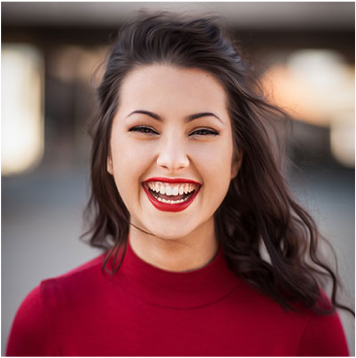
\includegraphics[width=1\textwidth]{images/vittoria.png}
\end{minipage}
\hspace{0.02\linewidth}
\begin{minipage}{0.65\textwidth}
	\textbf{Age:} 25 years-old \\
	\textbf{Gender:} Female\\
	\textbf{Profession:} Student\\
	\textbf{Education:} University student\\
	\textbf{Location:} Rome, Italy\\
	\textbf{Tecnology:} Mid level\\
	\textbf{Passions:} Watching movies and tv-series on streaming platforms \\
\end{minipage}

\paragraph{Persona}\mbox{}\\
Vittoria is 25 years-old and comes from Rome. She is a university student and in the free
time her main hobby is watching movies and tv-series on her favourite streaming platforms.
During her study breaks she likes to keep in touch with her friends on various social apps.

\paragraph{Scenario}\mbox{}\\
Vittoria has just terminated an intense study session and now she only wants to
relax watching a movie. She decides to call her best friend to spend the evening together.
Once she arrives, in order to choose which movie to watch, they both open the app to
compare their watchlists. After a while they realize that both have “La La Land“ in their
watchlists and so decide to watch it together.
At the end of the evening they both check it as “watched“ in their app.

\subsubsection{Persona 2 - Emanuele}

\begin{minipage}{0.3\textwidth}
	
\includegraphics[width=1\textwidth]{images/emanuele.png}
\end{minipage}
\hspace{0.02\linewidth}
\begin{minipage}{0.65\textwidth}
	\textbf{Age:} 33 years-old\\
	\textbf{Gender:} Male\\
	\textbf{Profession:} Programmer\\
	\textbf{Education:} Degree\\
	\textbf{Location:} Torino, Italy\\
	\textbf{Tecnology:} High level\\
	\textbf{Passions:} Action movies, technology\\
\end{minipage}

\paragraph{Persona}\mbox{}\\
Emanuele is 33 years-old and comes from Torino. He is a programmer and he likes
very much going to the cinema with his girlfriend.
As a programmer, he is addicted of technology in general, and more specific of mobile
devices; moreover he is a very organized guy, and so he likes to keep under control
everything he does in his life using mobile apps.

\paragraph{Scenario}\mbox{}\\
It is an afternoon autumn day. Emanuele and his girlfriend would have liked to go
out for a walk, but since it’s raining, they don’t know what to do. So, Emanuele opens
the app in search of new movies available in cinemas. In this list he founds that is just
available a new action movie with his favourite actor Vin Diesel; since also his
girlfriend likes action movies, they decide to go to the cinema to watch it and spend
a good afternoon together.


% Questionnaire  analysis -------------------------------------------------------------------------

\subsection{Questionnaire analysis}

Questionnaires are a useful method to investigate user needs, expectations, perspectives, priorities and preferences.
They are useful in user requirement but also in evaluation phase to investigate user satisfaction, user attitudes and opinions, relevance of collections and services to user needs, trends.
We designed the questionnaire in such a way that each question was clearly written, in order to not lead the user to a specific answer and to
always make them feel confortable while answering.
Below we present the questionnaire results used to better understand the target of potential users in order to have a better refinement of
some aspects of our application.
More precisely, we reached 151 people, and so we had a good number of answers, statistically speaking.\\

\paragraph{What's your age?}\mbox{}\\\\
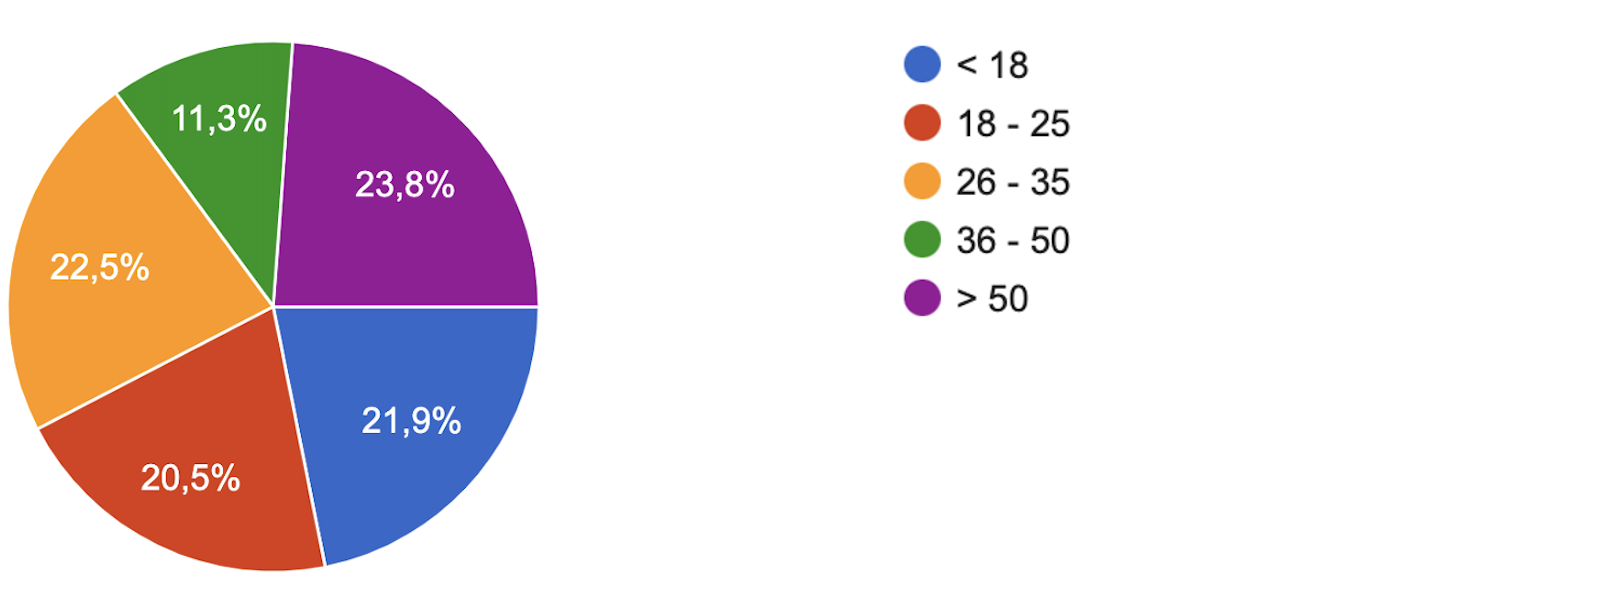
\includegraphics[width=0.7\textwidth]{Images/age.png}\\

\paragraph{What's your gender?}\mbox{}\\\\
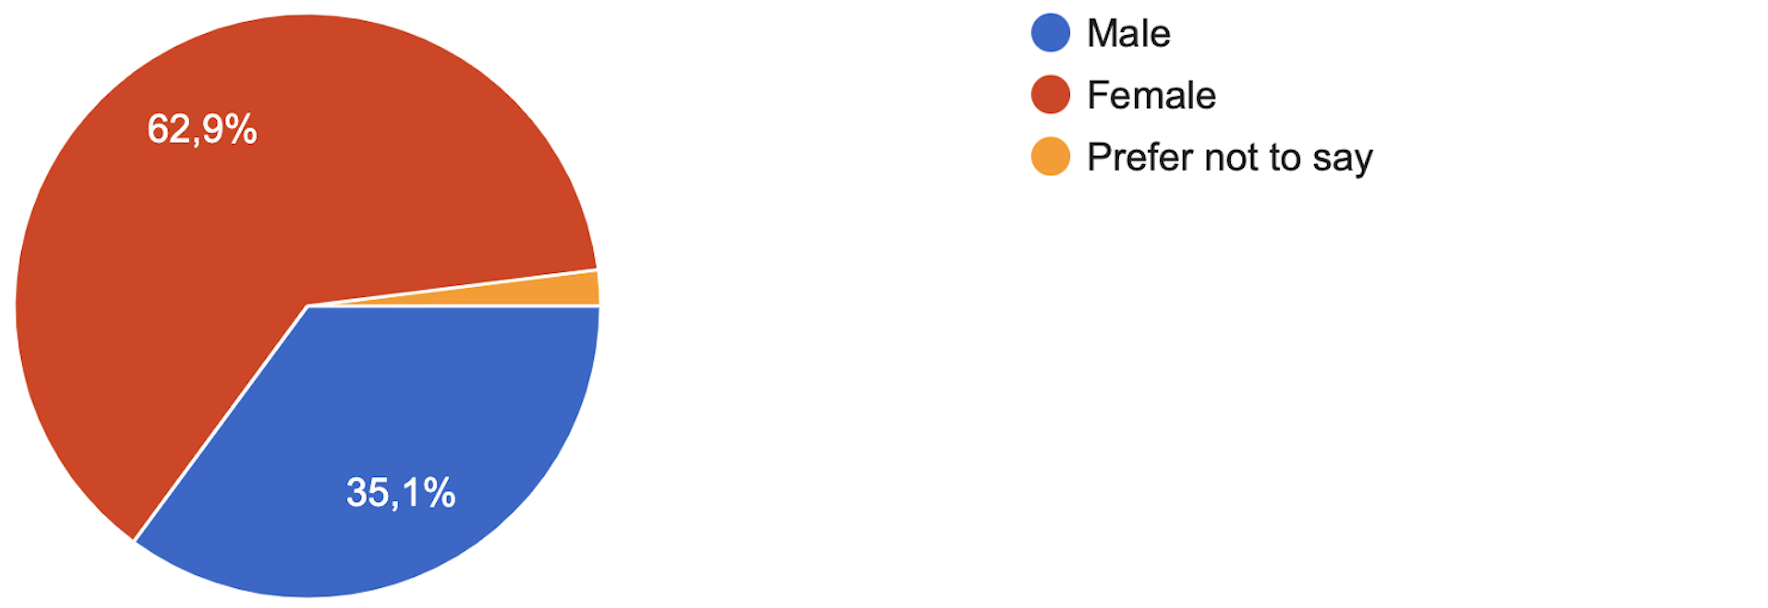
\includegraphics[width=0.7\textwidth]{Images/gender.png}\\

\paragraph{What's your educational level?}\mbox{}\\\\
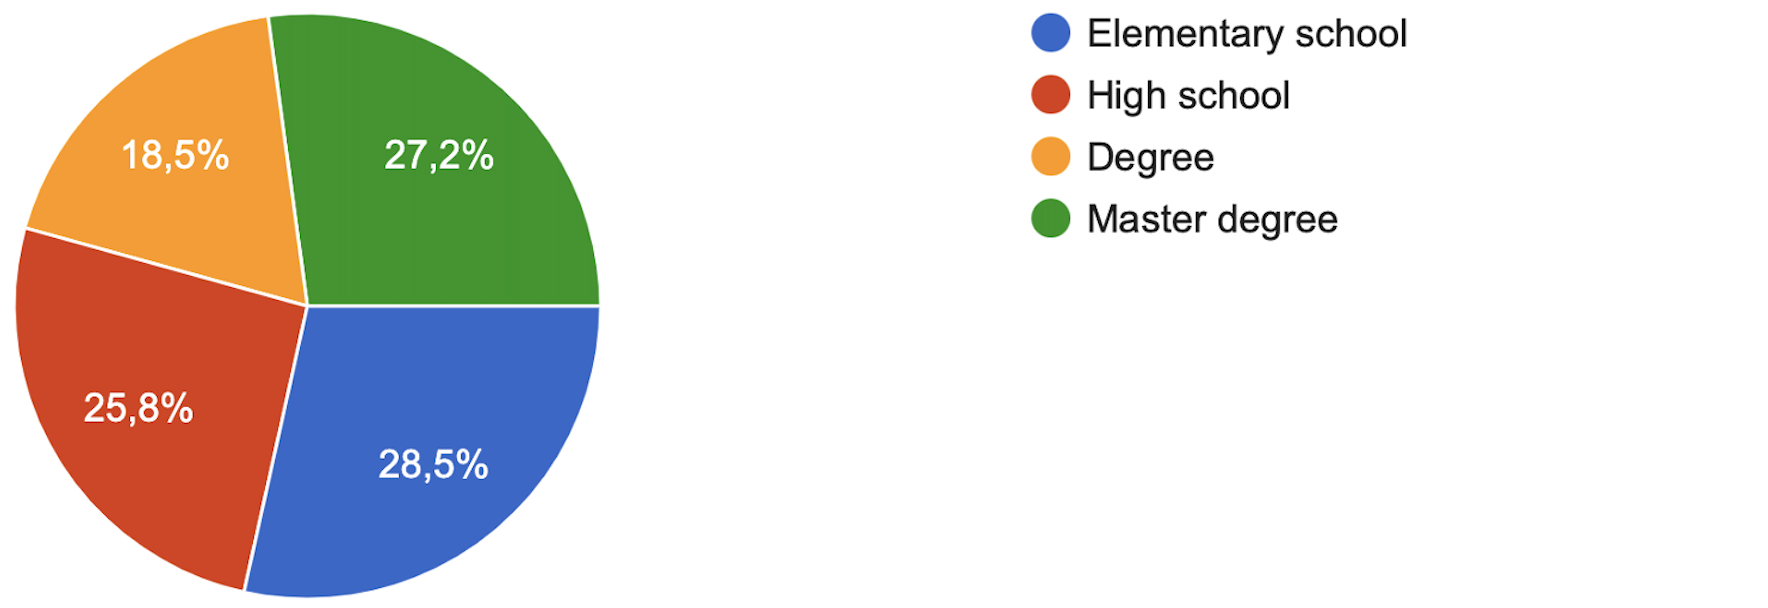
\includegraphics[width=0.7\textwidth]{Images/education.png}\\

\paragraph{How frequently do you use your smartphone on average?}\mbox{}\\\\
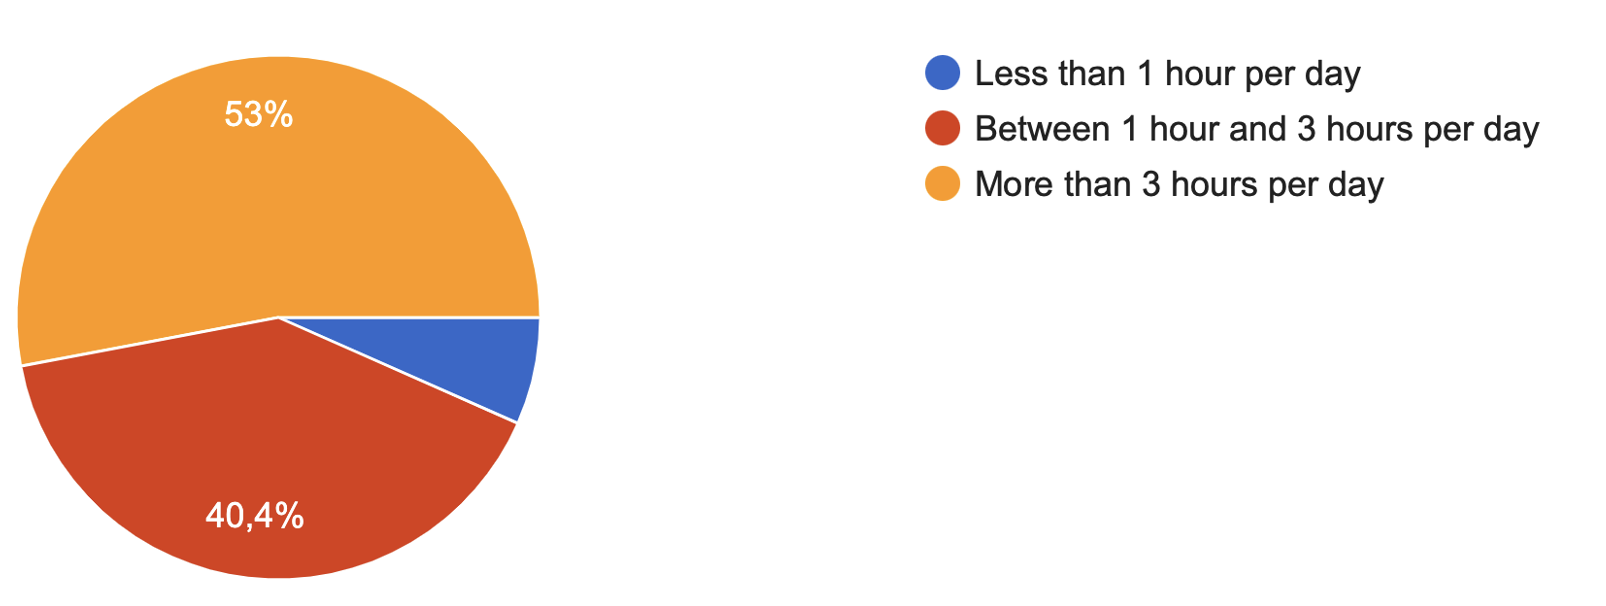
\includegraphics[width=0.7\textwidth]{Images/timeAtPhone.png}\\

\paragraph{How many times do you go to the cinema on average? (Before pandemic)}\mbox{}\\\\
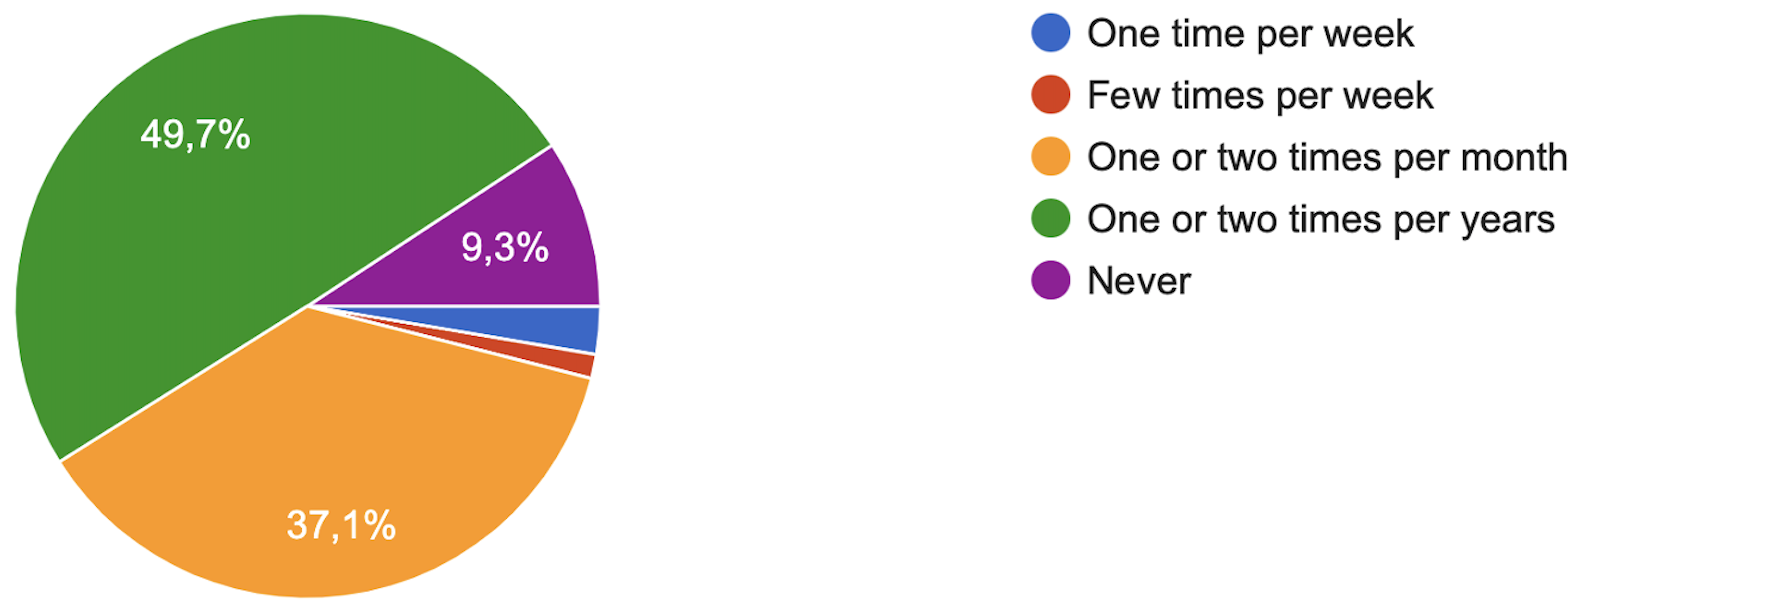
\includegraphics[width=0.7\textwidth]{Images/timeAtCinema.png}\\

\paragraph{How many times do you watch movies on streaming platforms/tv on average?}\mbox{}\\\\
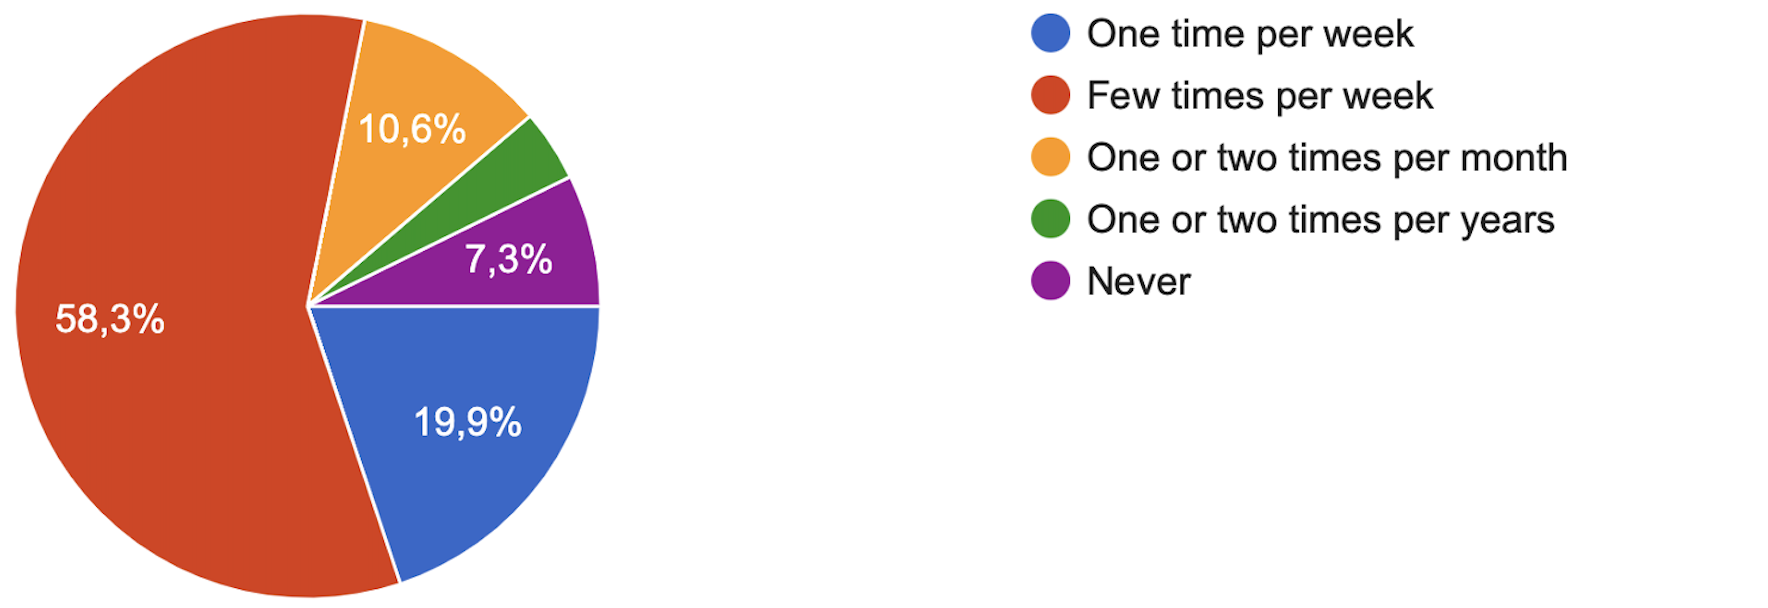
\includegraphics[width=0.7\textwidth]{Images/timeStreaming.png}\\

\paragraph{Which streaming platforms do you know?}\mbox{}\\\\
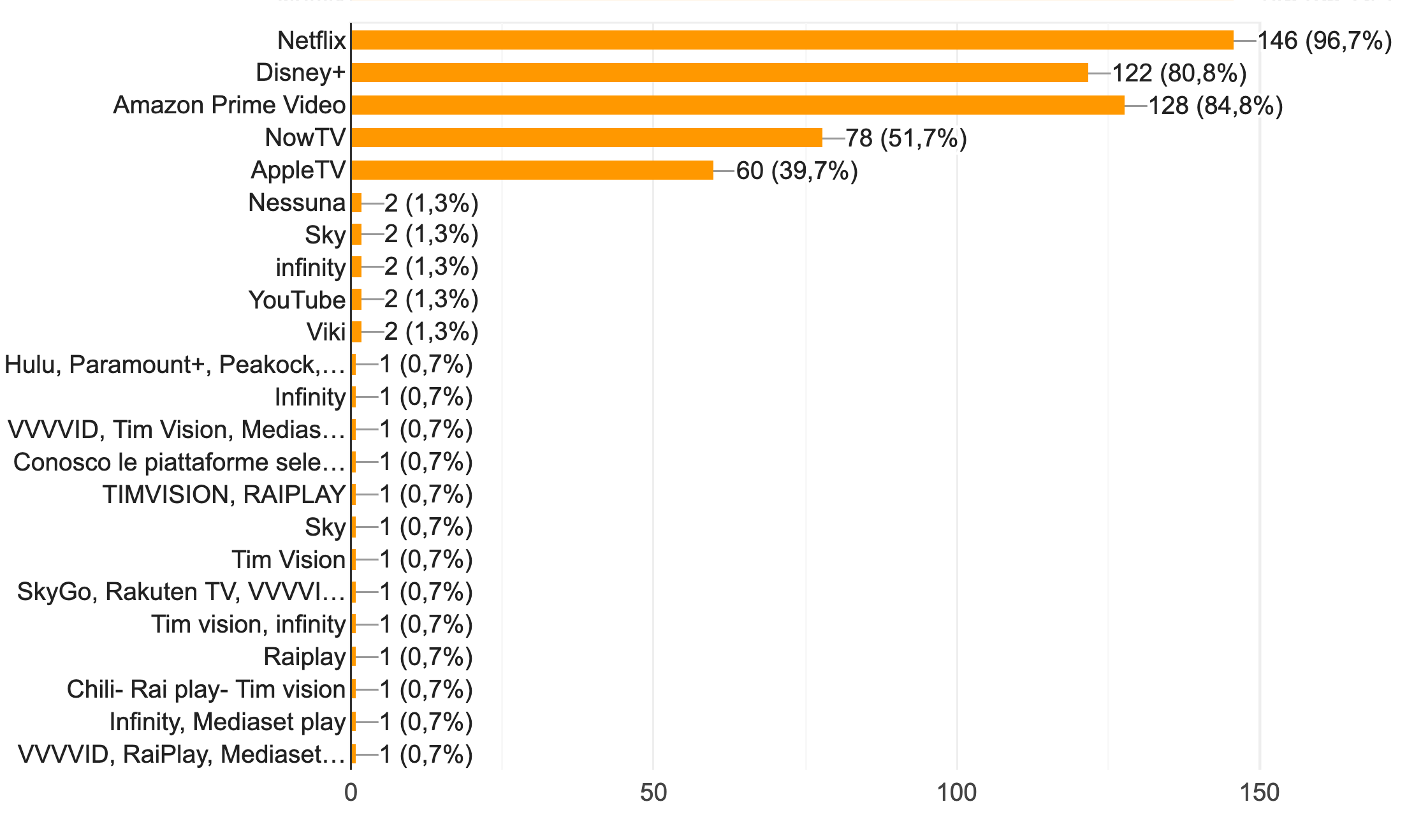
\includegraphics[width=1\textwidth]{Images/streamingPlatform.png}\\\\

\paragraph{Which streaming platforms do you use?}\mbox{}\\\\
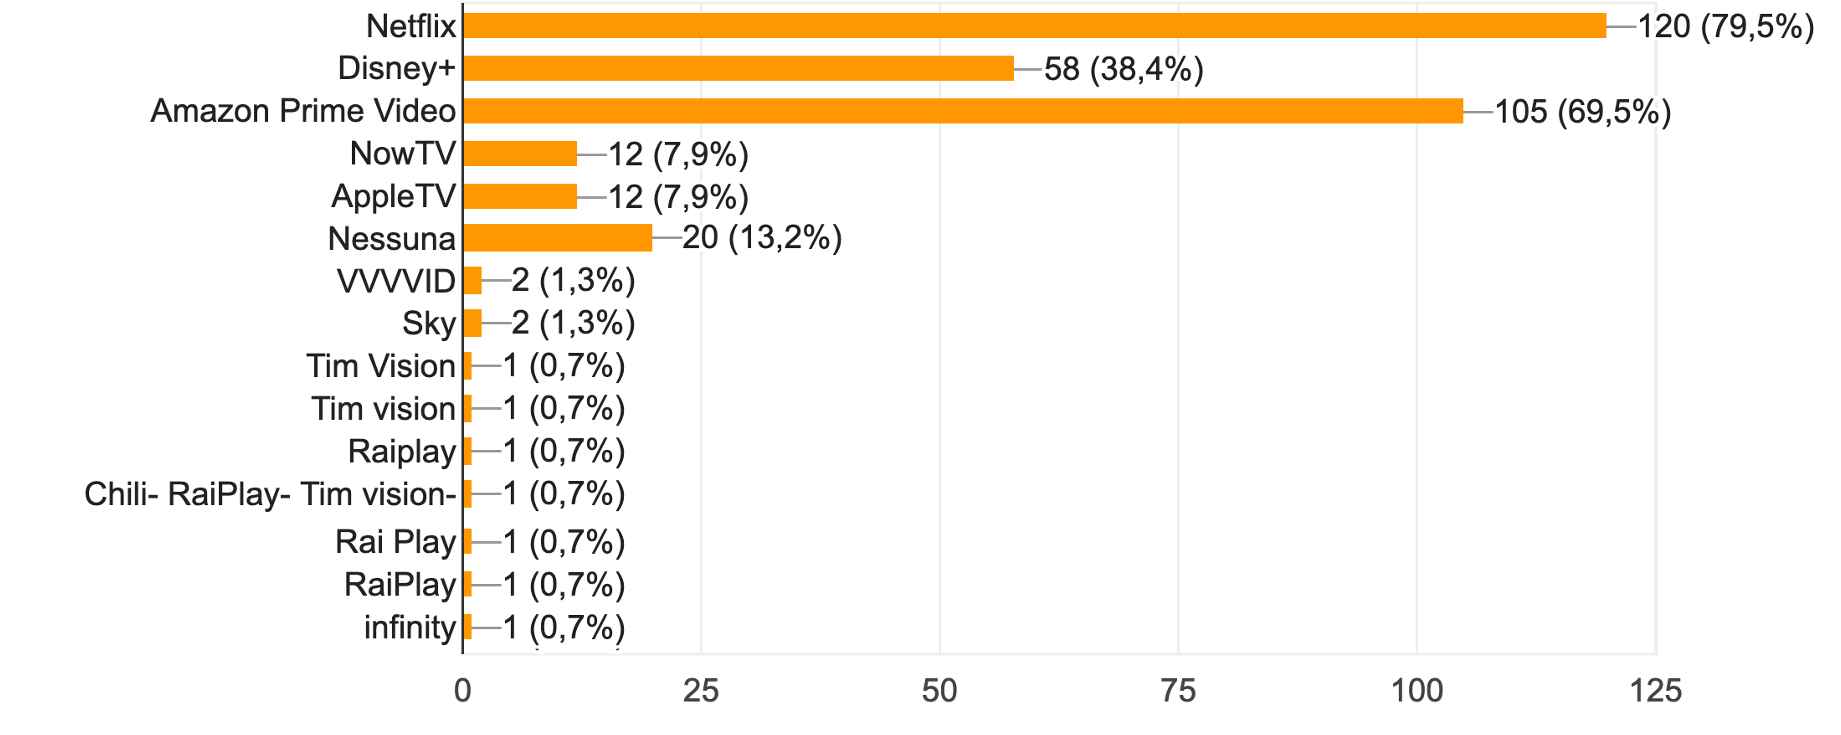
\includegraphics[width=1\textwidth]{Images/streamingPlatformUsed.png}\\

\paragraph{Do you use any movies related app?}\mbox{}\\\\
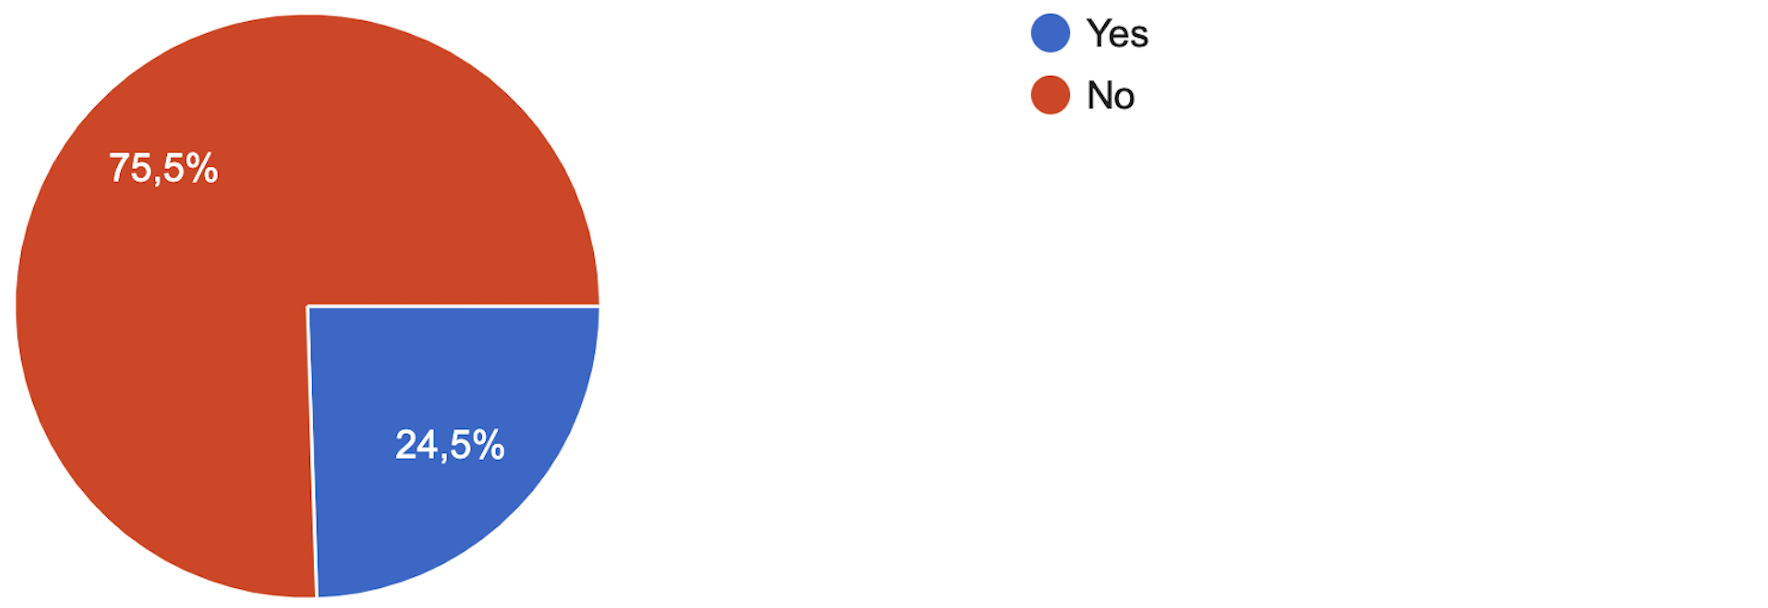
\includegraphics[width=0.7\textwidth]{Images/app.png}\\

\paragraph{If you use any movies related app, which one?}\mbox{}\\\\
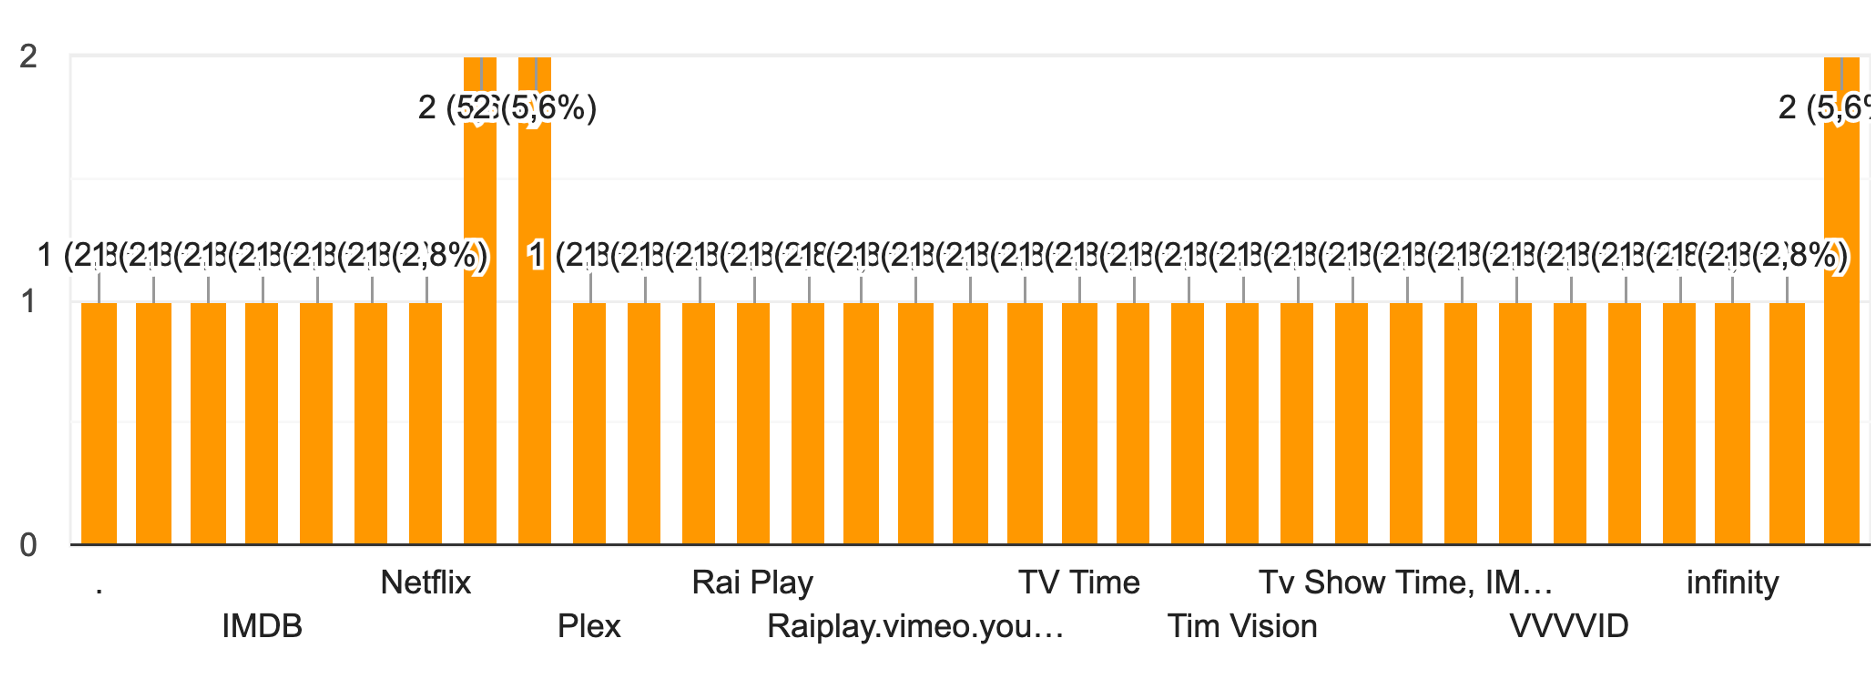
\includegraphics[width=1\textwidth]{images/appUsed.png}\\\\\\\\

\paragraph{If you don't use any movies related app, how much would you be interest in using one?}\mbox{}\\\\
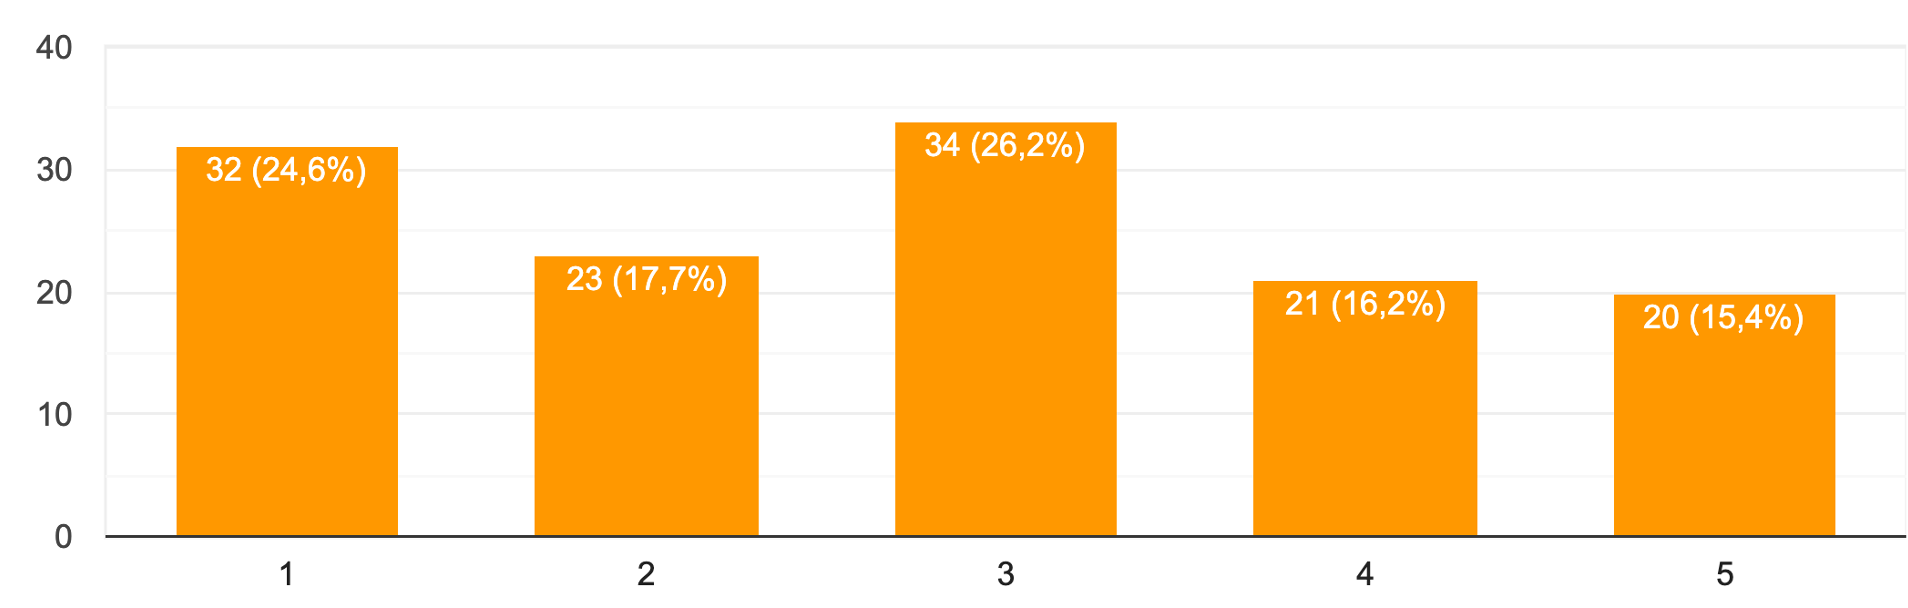
\includegraphics[width=1\textwidth]{images/interesting.png}\\

\paragraph{How much do you think the following features are important in such an app?}\mbox{}\\\\
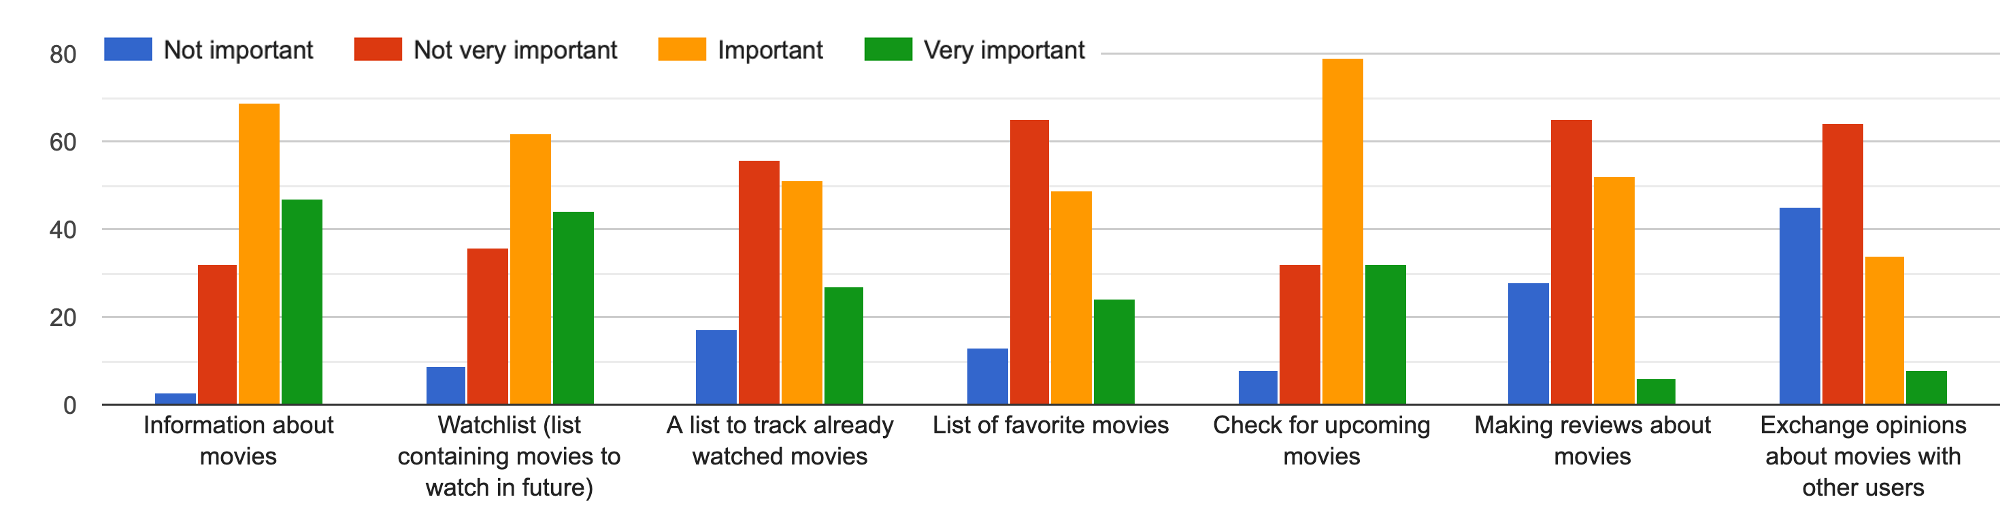
\includegraphics[width=1\textwidth]{Images/features.png}\\

\subsubsection{Conclusions}
After having analyzed the results obtained from the questionnaires, we have formalized the following conclusions:
\begin{itemize}
	\item {Regarding ages, we noticed that there is no predominant range, but they 
	are more or less equally distributed between 18 and 50, and the majority 
	of them are women.}
	\item {The majority of them uses smartphone more than 3 hours per day.}
	\item {Since we noticed that the majority of people rarely goes to cinema and 
	conversely watches very often movies on streaming platform, we decided to focus 
	our app on this feature.}
	\item {Moreover, given the fact that a very high number of people does not use 
	a movie related app and that the majority of them would be interested in doing 
	this, we thought that the idea of such an app would be very appreciated.}
	\item {Finally, from the last question, emerge the most wanted features such 
	as have informations about movies, have the possibility to add movies to lists 
	and have informations about upcoming movies, and so we decided to focused on them.}
\end{itemize}



% Task analysis: HTA and STN -------------------------------------------------------------------------

\newpage

\section{Task analysis: HTA and STN}

In this section we are going to show HTA and STN in order to formalize the main task of 
our application and to analyze and describe how users can reach their goals.\\
\textit{Hierarchical Task Analysis} (HTA) is a task description methodology that is used to produce a 
complete description of tasks in a hierarchical structure of goals, sub-goals, operations and plans 
in order to have a complete representation of the action.\\
Instead, a \textit{State Transition Network} (STN) represents a dialogue between the user and the system, 
in which the system could support the tasks that the customer has to execute.
It describes which are the available actions at a certain point, and the consequent 
state that the system will reach.\\\\
The main tasks that the user can do in our application are:
\begin{itemize}
	\item Login into the app.
	\item Search for a movie, an actor or movie director.
	\item Add a movie into three lists: watchlist, movie already watched list and favourite movie list.
	\item Make a review regarding a movie.
	\item Interact with other users by commenting a review written by another user.
\end{itemize}
\hbox{}
\subsection{Login}
The user can login into the app if registered, either through online platforms (Google, Facebook) 
or using his personal email and password, in order to save in the cloud all his data regarding the app. 
From now on, in the following HTAs, we assume that the user is logged in.\\ 

\paragraph{HTA - Login}\mbox{}\\
\begin{figure}[H]
	\centering
	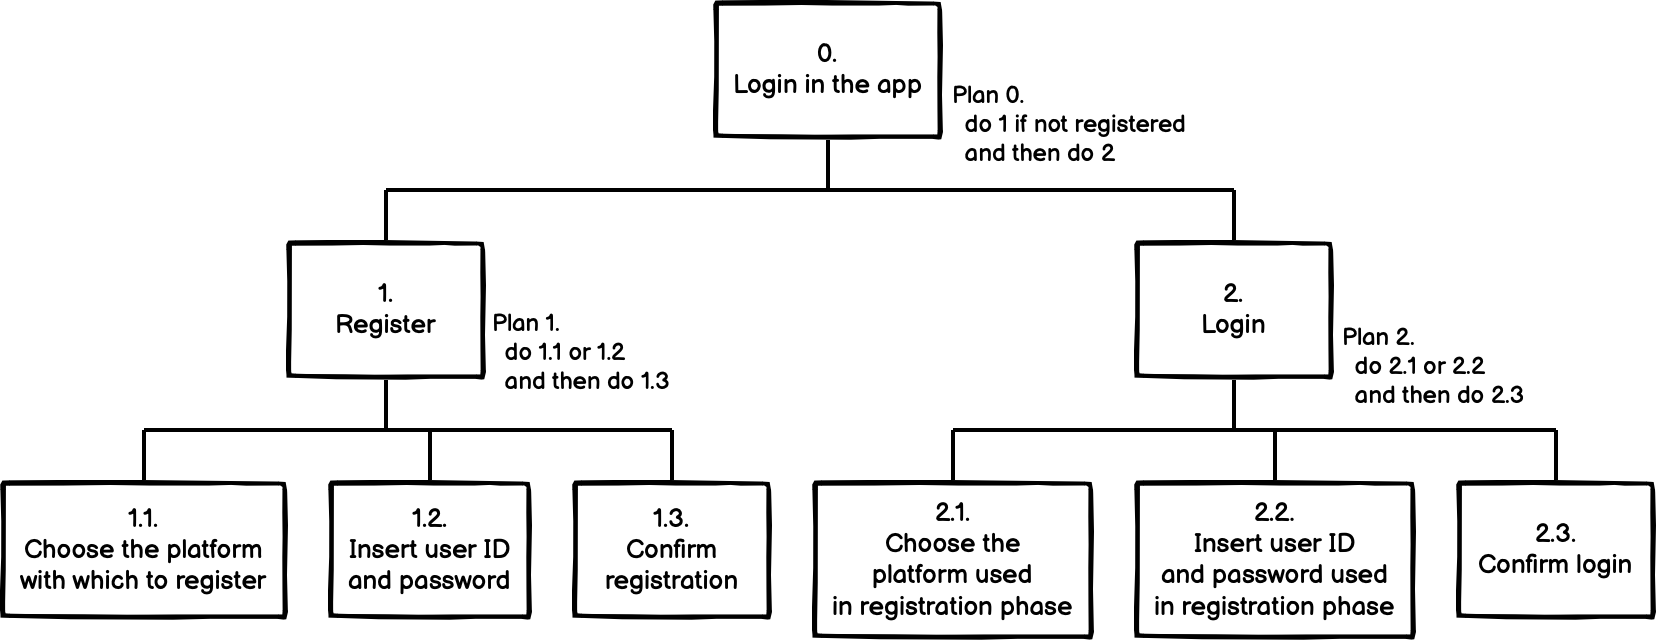
\includegraphics[width=1\textwidth]{images/Login HTA.png}\\
\end{figure}
\mbox{}\\\\
\paragraph{STN - Login}\mbox{}\\
\begin{figure}[H]
	\centering
	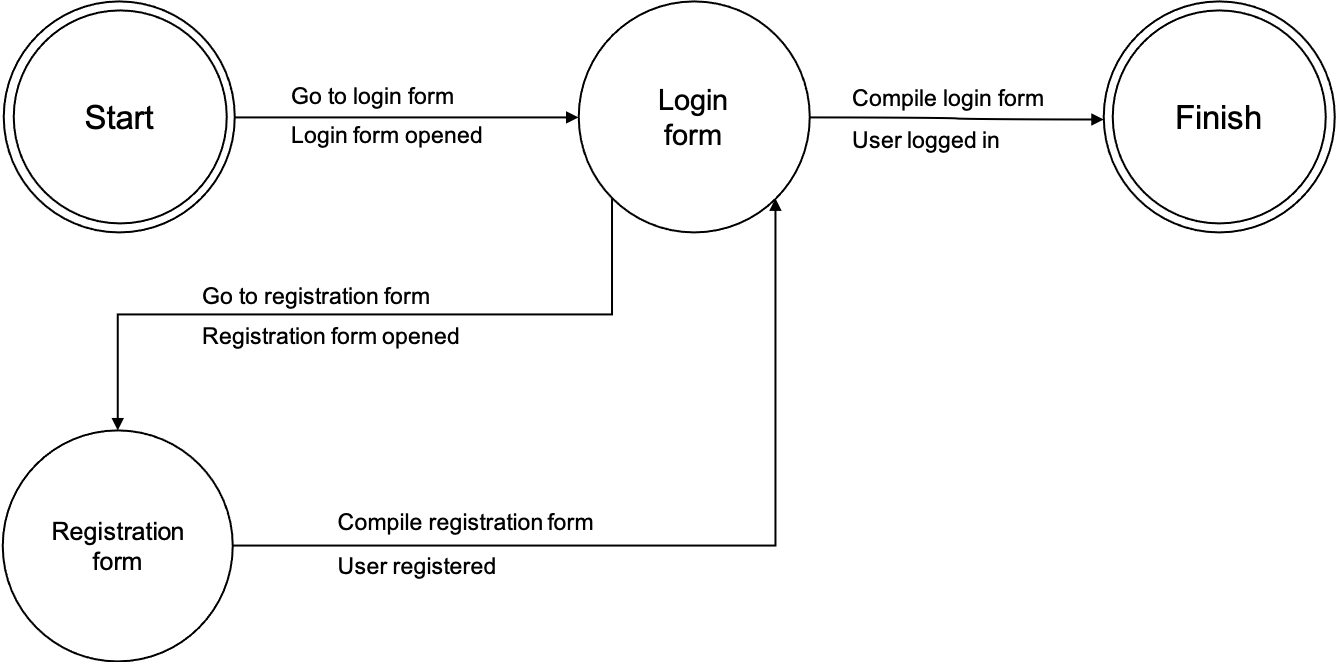
\includegraphics[width=0.9\textwidth]{images/LoginSTN.png}\\
\end{figure}

\mbox{}\\

\subsection{Search for a movie or a person}
The user searches for the movie or the person he wants to know information about. 
He can do search by title, actor or movie director and, when the results are shown, 
he selects the result he is interested in.\\ 

\paragraph{HTA - Search for a movie or a person}\mbox{}\\
\begin{figure}[H]
	\centering
	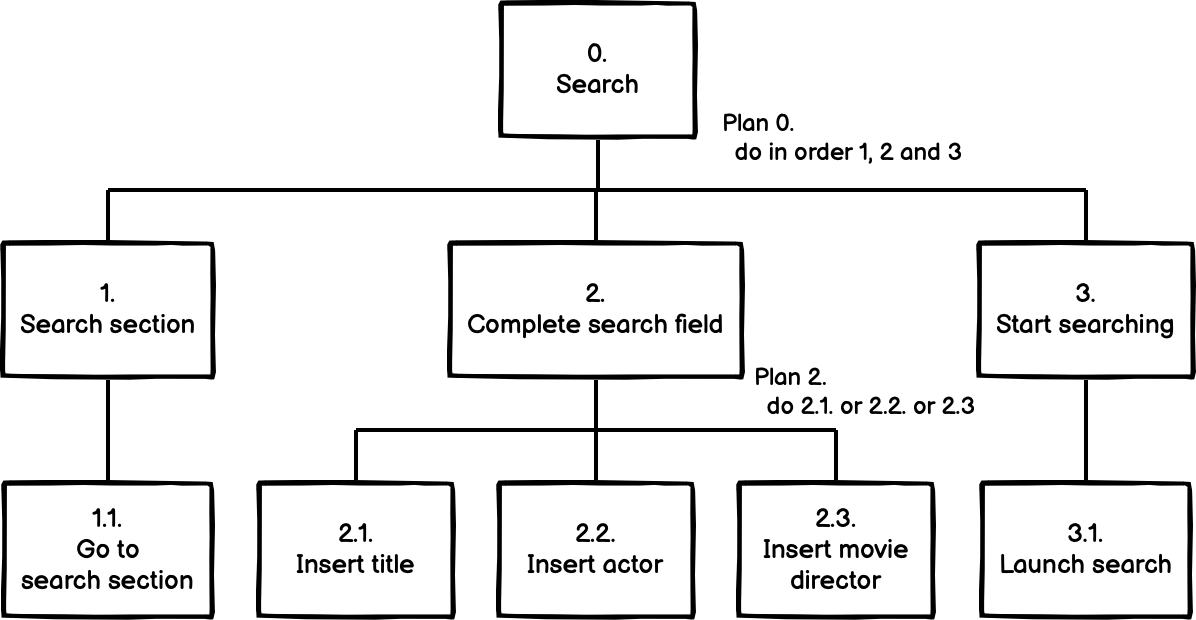
\includegraphics[width=1\textwidth]{images/Search HTA.png}\\
\end{figure}
\mbox{}\\
\paragraph{STN - Search for a movie or a person}\mbox{}\\
\begin{figure}[H]
	\centering
	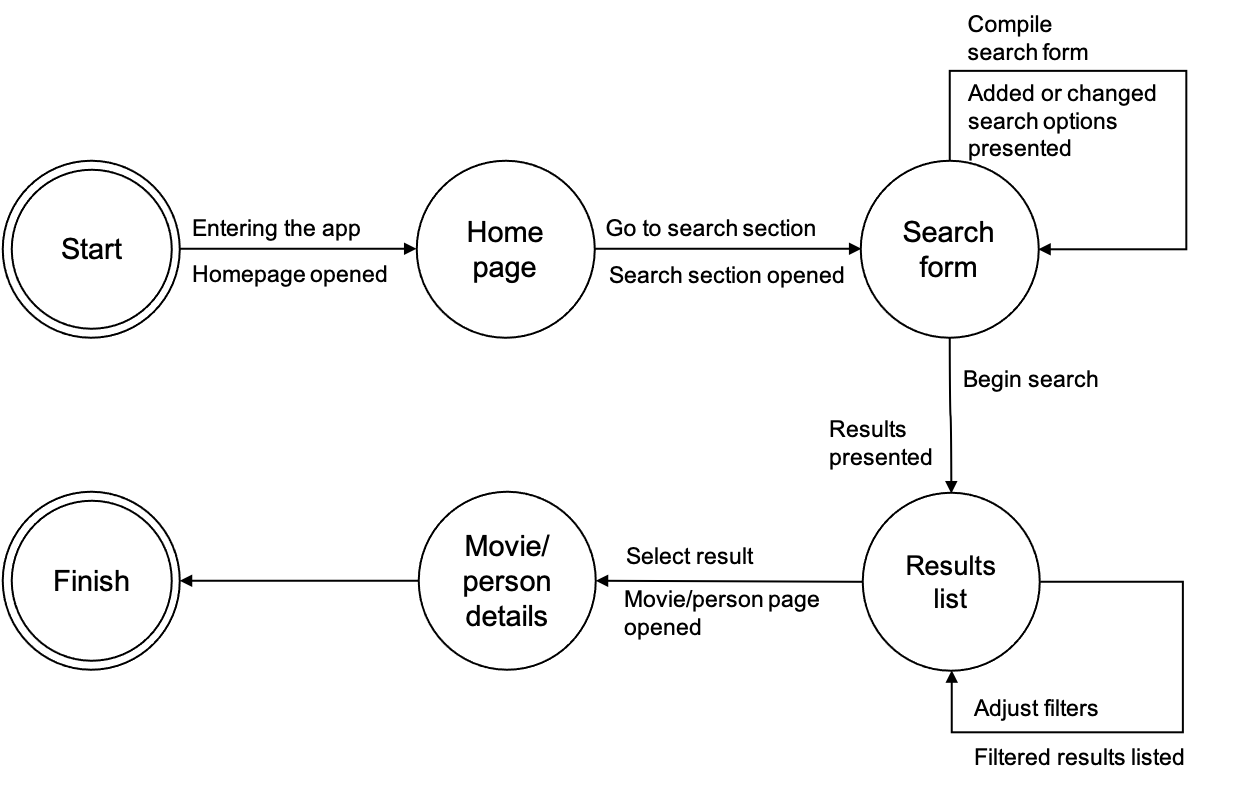
\includegraphics[width=1\textwidth]{images/SearchSTN.png}\\
\end{figure}

\subsection{Add movie to a list}
The user can add a movie into a list: he can choose between a watchlist that contains movies to watch 
in the future, a list containing movies already watched and a list containing favourite movies. 
We are assuming that the user has already selected a movie.

\paragraph{HTA - Add movie to a list}\mbox{}\\
\begin{figure}[H]
	\centering
	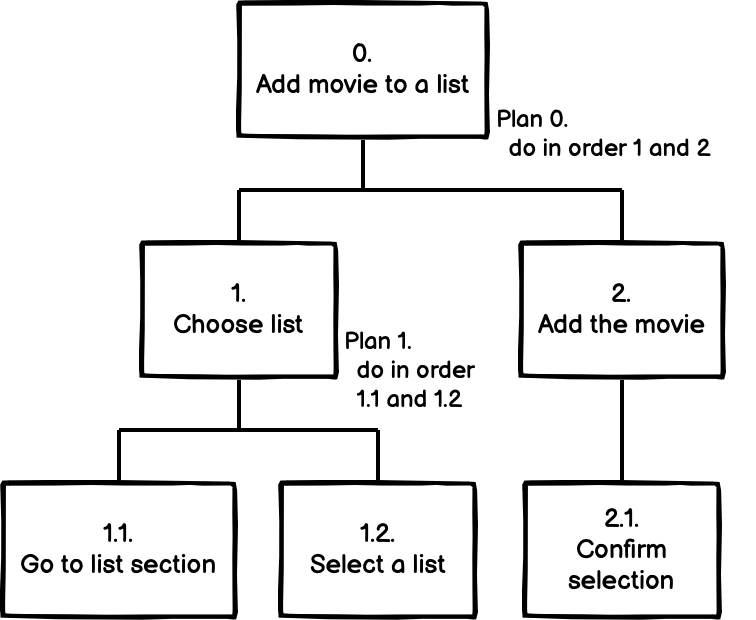
\includegraphics[width=0.6\textwidth]{images/Add movie HTA.png}\\
\end{figure}

\paragraph{STN - Add movie to a list}\mbox{}\\
\begin{figure}[H]
	\centering
	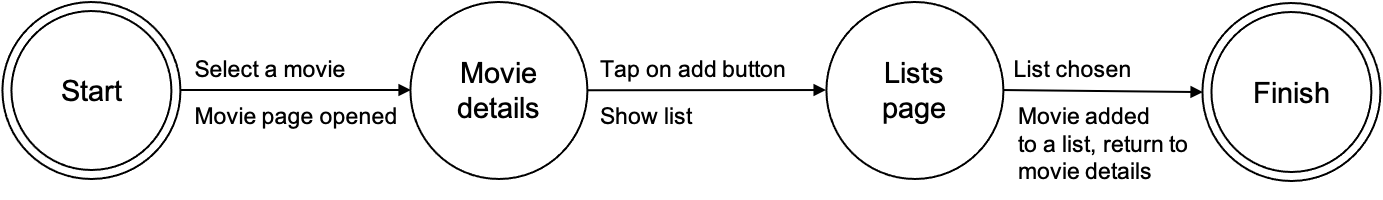
\includegraphics[width=1\textwidth]{images/AddMovieSTN.png}\\
\end{figure}

\mbox{}\\

\subsection{Make a review}
The user can make a review regarding a movie. In particular, once he selected a movie, 
he can go to the review page either from the movie page or from the page containing all reviews.\\ 

\paragraph{HTA - Make a review}\mbox{}\\
\begin{figure}[H]
	\centering
	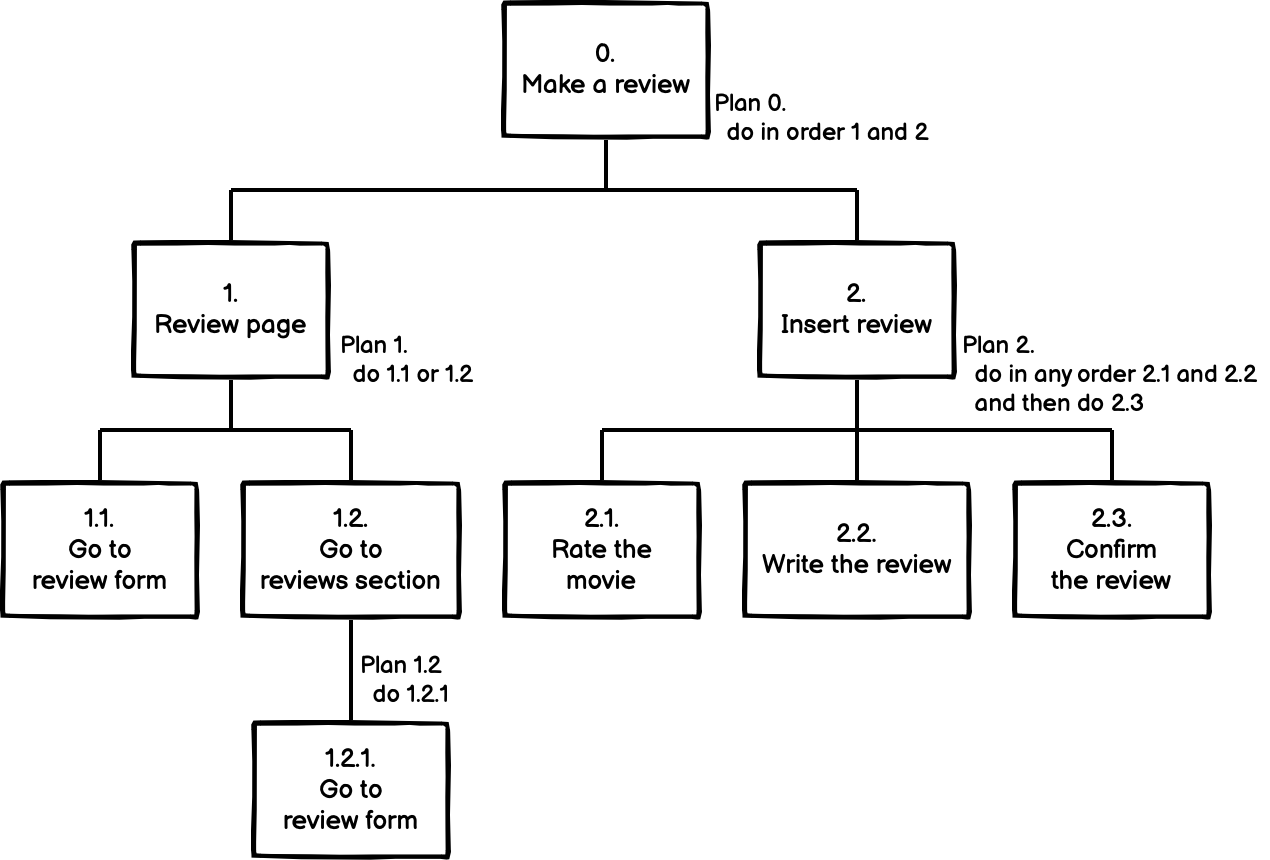
\includegraphics[width=1\textwidth]{images/Make a review HTA.png}\\
\end{figure}
\mbox{}\\\\\\
\paragraph{STN - Make a review}\mbox{}\\
\begin{figure}[H]
	\centering
	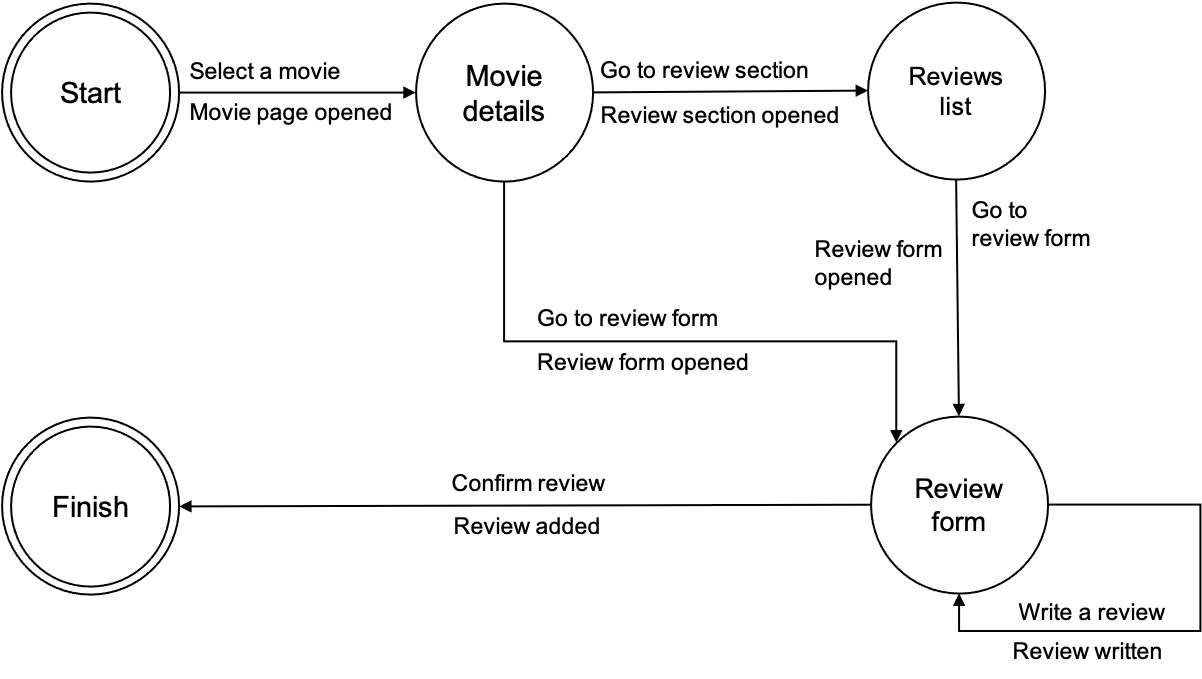
\includegraphics[width=1\textwidth]{images/MakeAReviewSTN.png}\\
\end{figure}


\subsection{Comment other users’ reviews }
The user can comment a review written by another user. In particular he can go to the page containing 
all the reviews, choose one of them and comment it.\\

\paragraph{HTA - Comment other users’ reviews}\mbox{}\\
\begin{figure}[H]
	\centering
	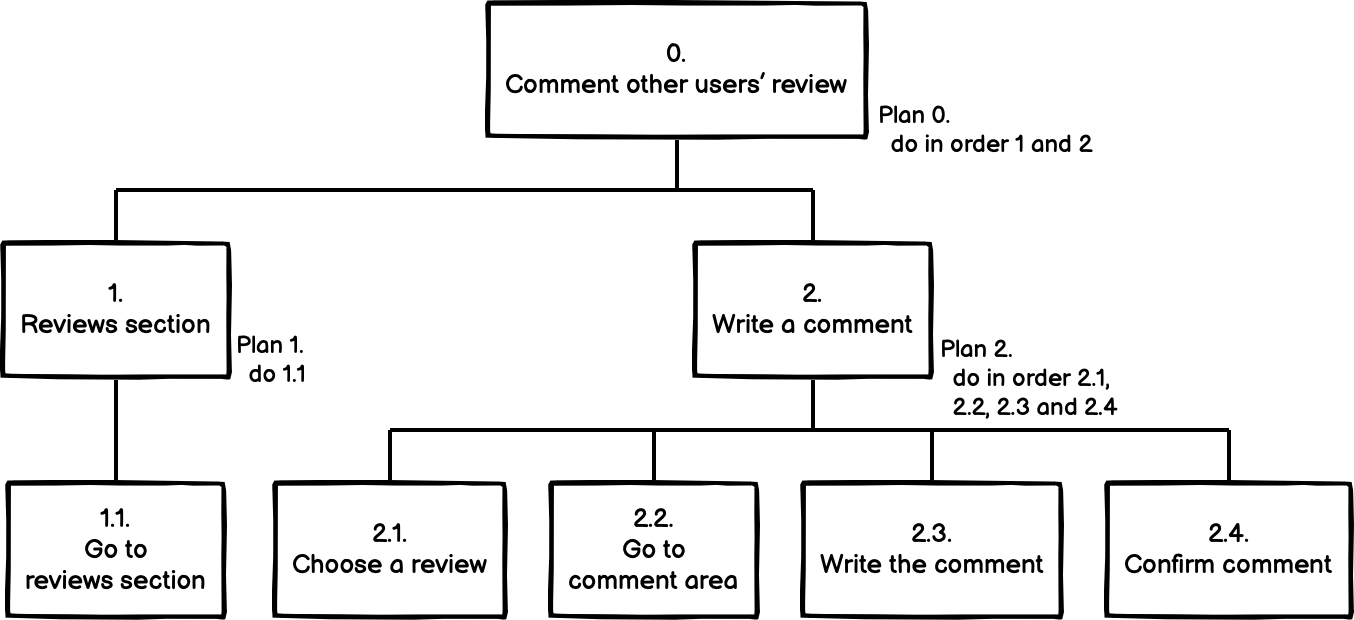
\includegraphics[width=1\textwidth]{images/Comments HTA.png}\\
\end{figure}
\mbox{}\\
\paragraph{STN - Comment other users’ reviews}\mbox{}\\
\begin{figure}[H]
	\centering
	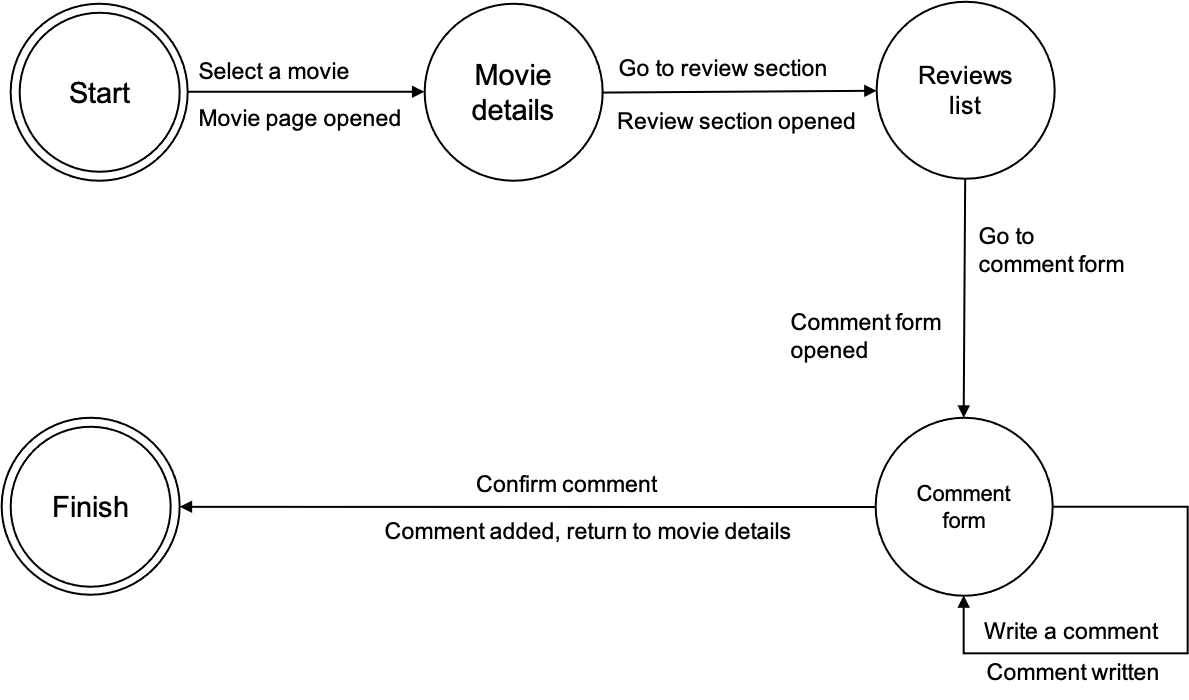
\includegraphics[width=1\textwidth]{images/CommentsSTN.png}\\
\end{figure}

% Mockup and prototype 0 -------------------------------------------------------------------------

\newpage

\section{Prototype 0: mockups}
In this section we are going to present our first prototype realized through mockups
in Balsamiq Wireframes. In the first prototype we created the skeleton of the application
by modeling the different screens and the interaction between them.\\\\ 
The main functionalities of this prototype are:
\begin{itemize}
	\item Login and registration of an user.
	\item Search for a movie or a person.
	\item Add a movie to a list.
	\item Review a movie.
	\item Comment other reviews.
\end{itemize}

\paragraph{Login and Registration}
\mbox{}
\begin{figure}[H]
	\centering
	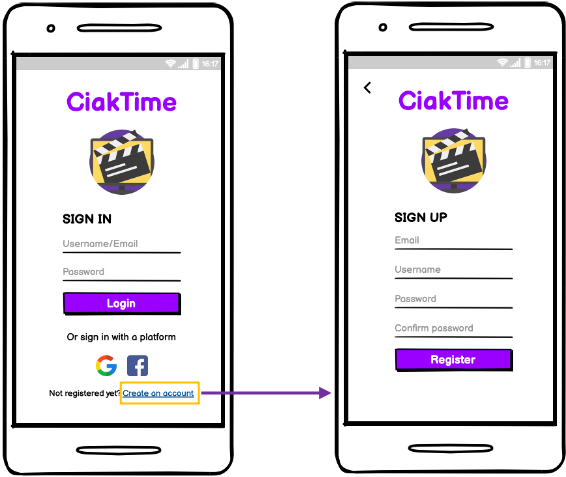
\includegraphics[width=0.5\textwidth]{images/mockups/signInSignUp.png}\\
	\caption{Login and Registration pages}
\end{figure}
\begin{figure}[H]
	\centering
	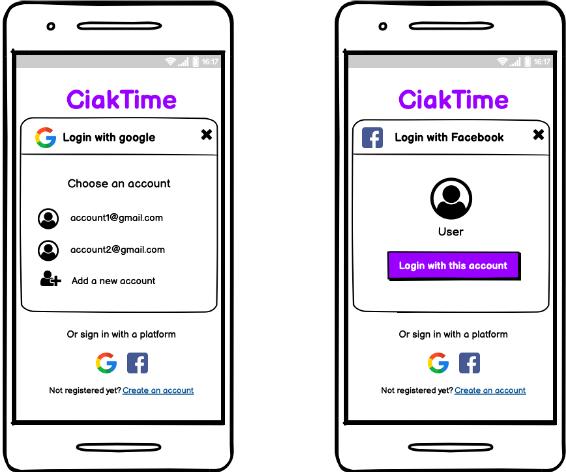
\includegraphics[width=0.5\textwidth]{images/mockups/loginSocial.png}\\
	\caption{Login with Google and Facebook}
\end{figure}
\paragraph{Search for a movie or a person}
\mbox{}\\\\
The user can do the search by tapping on the search bar and, if he wants, he can apply filters by tapping 
on the proper icon.\\
\begin{figure}[H]
	\centering
	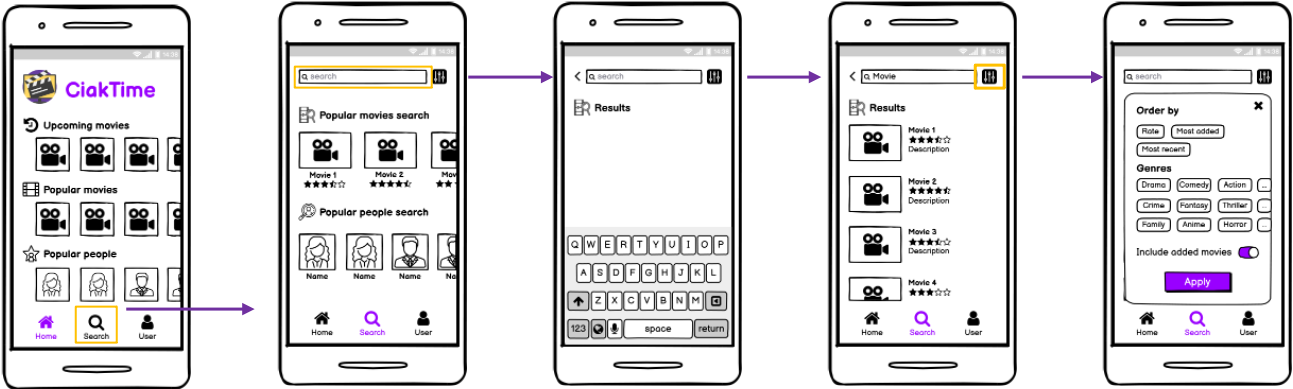
\includegraphics[width=1\textwidth]{images/mockups/search2.png}\\
	\caption{Searching process with optional filters}
\end{figure}
\mbox{}\\
\noindent
After having searched for a movie or a person, the user can tap on it and the application, according
to his choice, will show one of the following screens:
\begin{center}
	\begin{minipage}{0.4\textwidth}
		\begin{figure}[H]
			\centering
			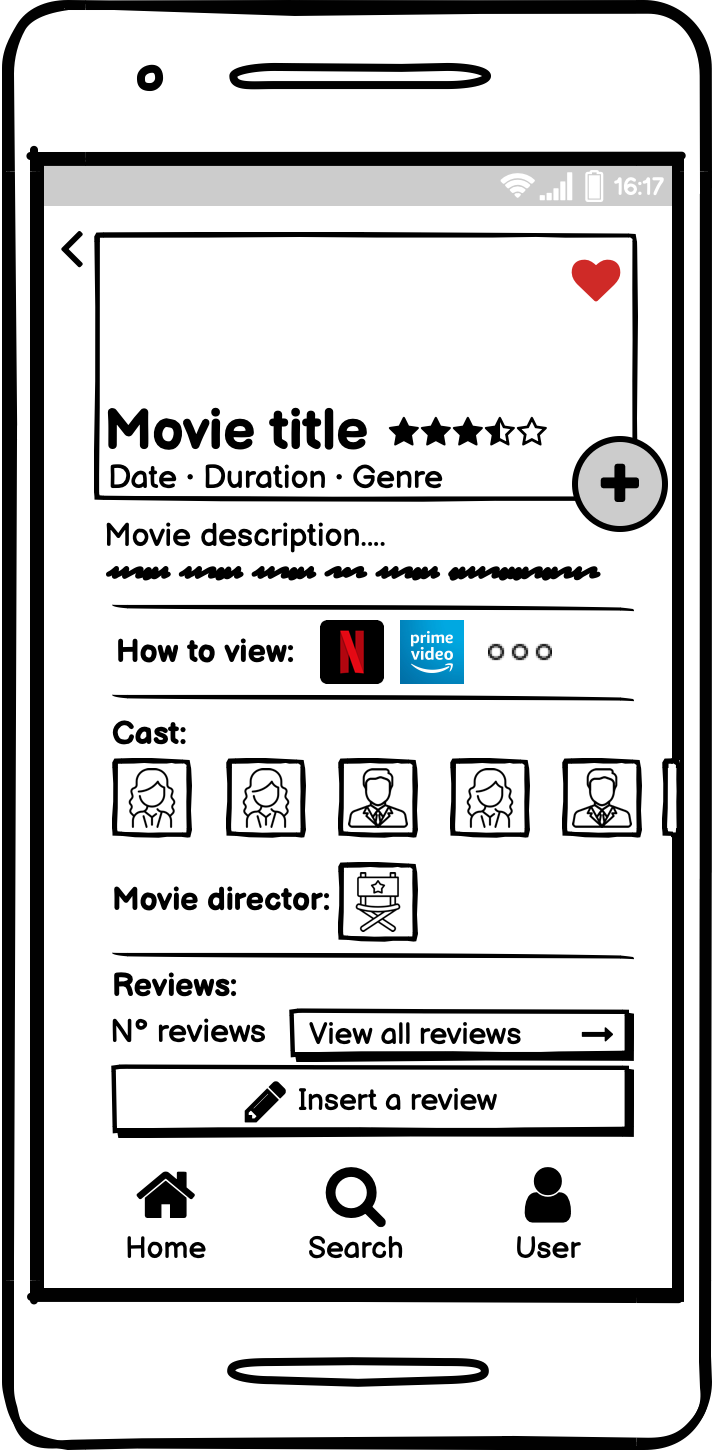
\includegraphics[width=0.5\textwidth]{images/mockups/Movie page.png}\\
			\caption{Movie page}
		\end{figure}
	\end{minipage}
	\hspace{0.01\linewidth}
	\begin{minipage}{0.4\textwidth}
		\begin{figure}[H]
			\centering
			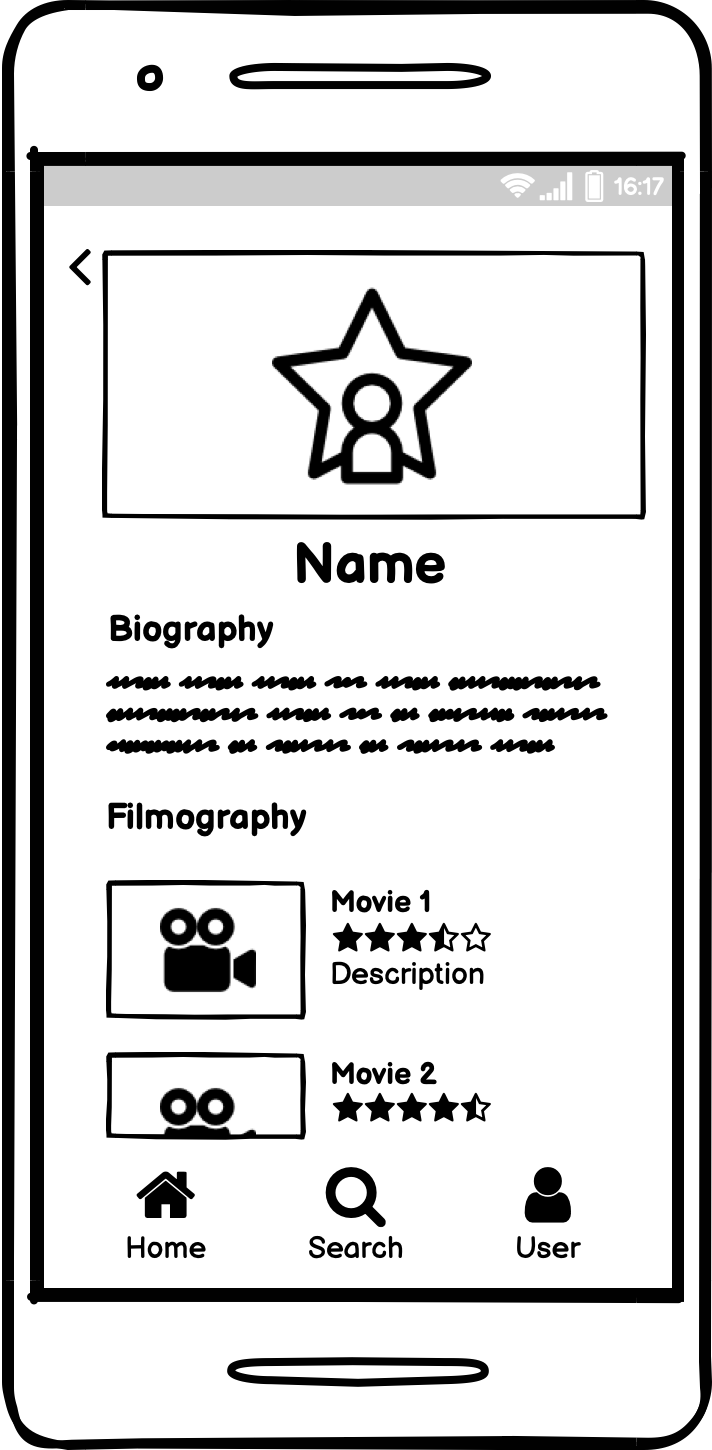
\includegraphics[width=0.5\textwidth]{images/mockups/People page.png}\\
			\caption{Person page}
		\end{figure}
	\end{minipage}	
\end{center}
\mbox{}\\\\\\\\\\\\\\\\\\\\
\paragraph{Add a movie to a list}
\mbox{}\\\\
The user can add a movie to a list in the following ways: by tapping on the "+" button to add the movie to 
"Watchlist" or "Already watched" and by tapping on the heart icon to add the movie to "Favourite movies".
\mbox{}
\begin{figure}[H]
	\centering
	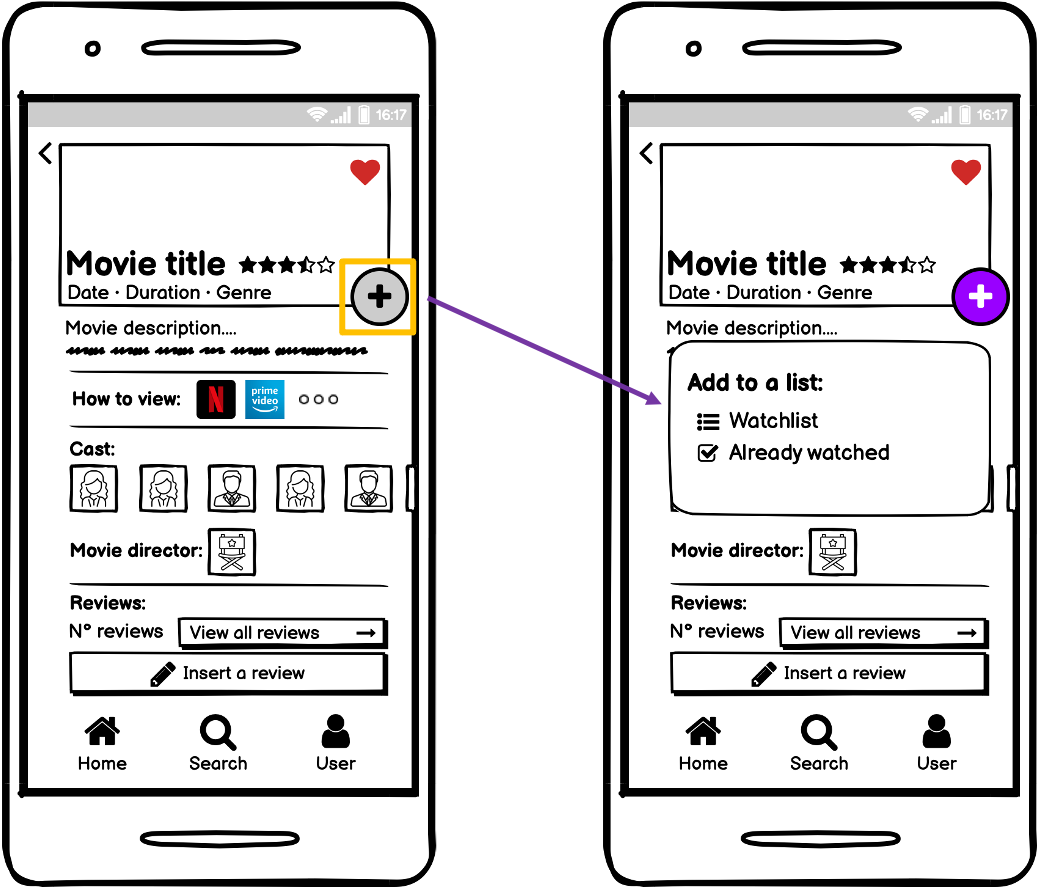
\includegraphics[width=0.5\textwidth]{images/mockups/addMovie.png}\\
	\caption{Add a movie to a list process}
\end{figure}
\noindent
The user can reach the lists where he added the movie from the user profile page,
in order to see all the movies added in watchlist, already watched list and favourite movies list.\\
\begin{figure}[H]
	\centering
	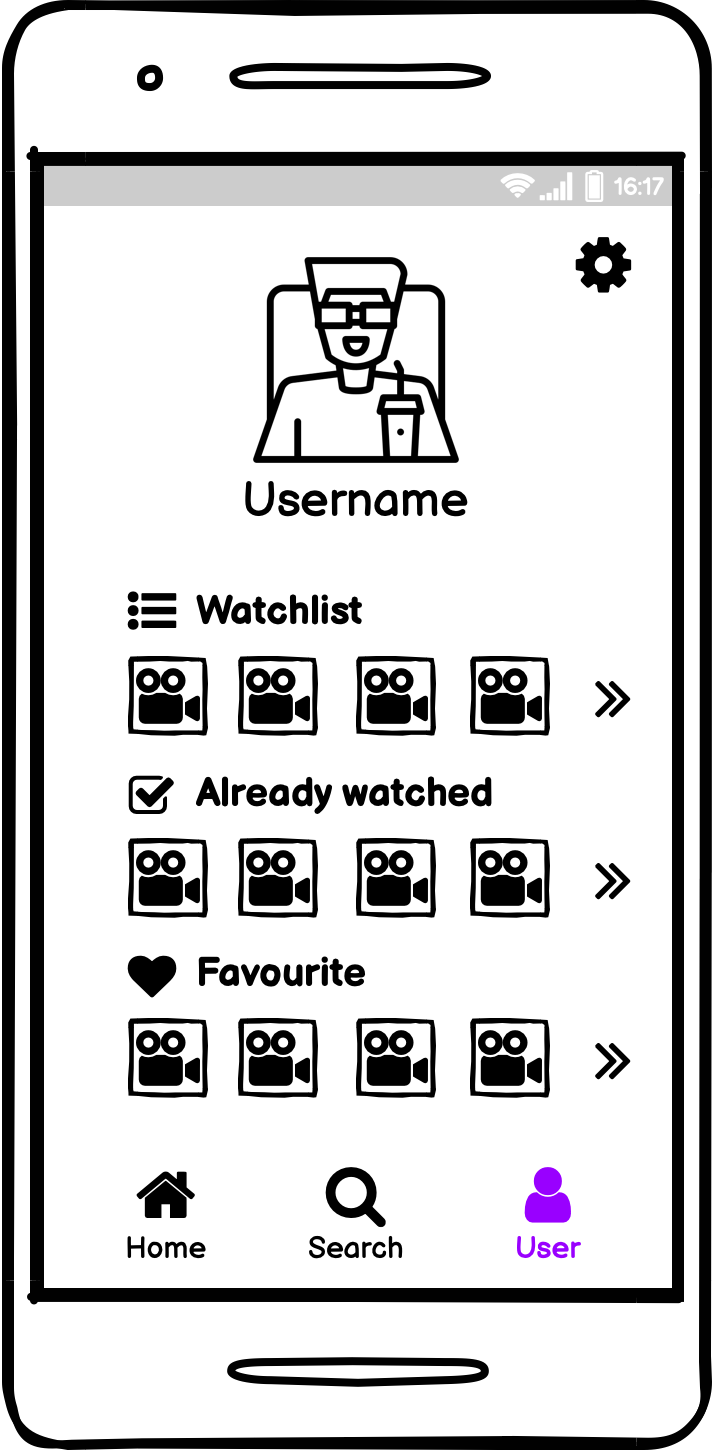
\includegraphics[width=0.21\textwidth]{images/mockups/User profile.png}\\
	\caption{User profile page}
\end{figure}
\begin{center}
	\begin{minipage}{0.31\textwidth}
		\begin{figure}[H]
			\centering
			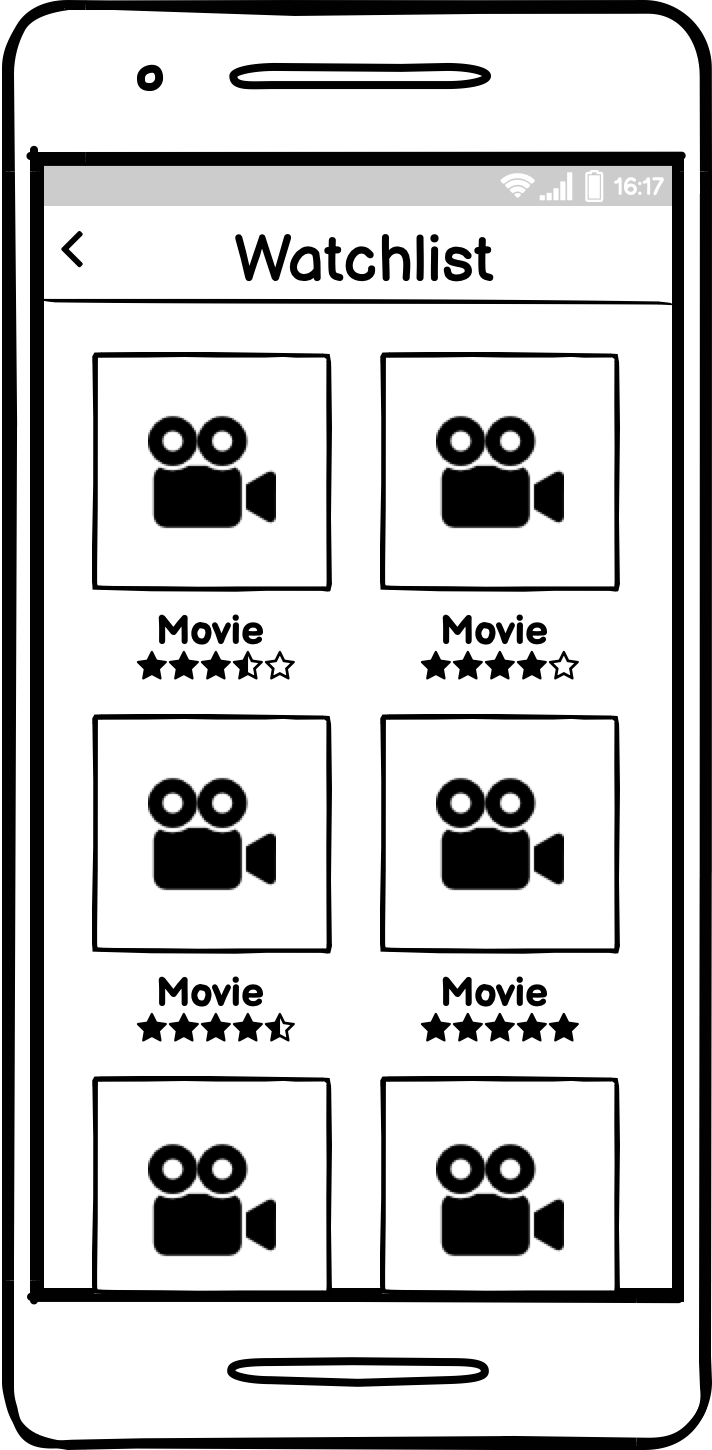
\includegraphics[width=0.68\textwidth]{images/mockups/Watchlist.png}\\
			\caption{Watchlist}
		\end{figure}
	\end{minipage}
	\hspace{0.01\linewidth}
	\begin{minipage}{0.33\textwidth}
		\begin{figure}[H]
			\centering
			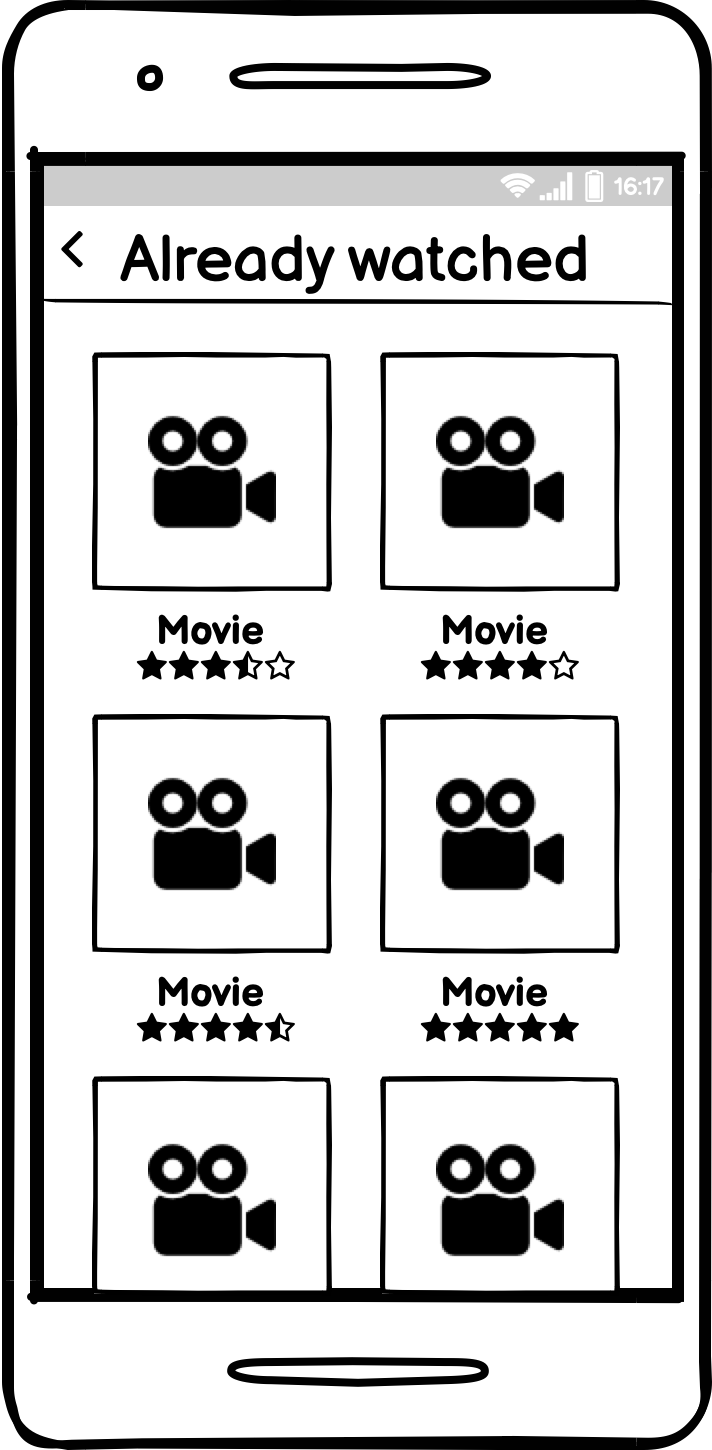
\includegraphics[width=0.65\textwidth]{images/mockups/Already watched.png}\\
			\caption{Movie already watched}
		\end{figure}
	\end{minipage}
	\hspace{0.01\linewidth}
	\begin{minipage}{0.31\textwidth}
		\begin{figure}[H]
			\centering
			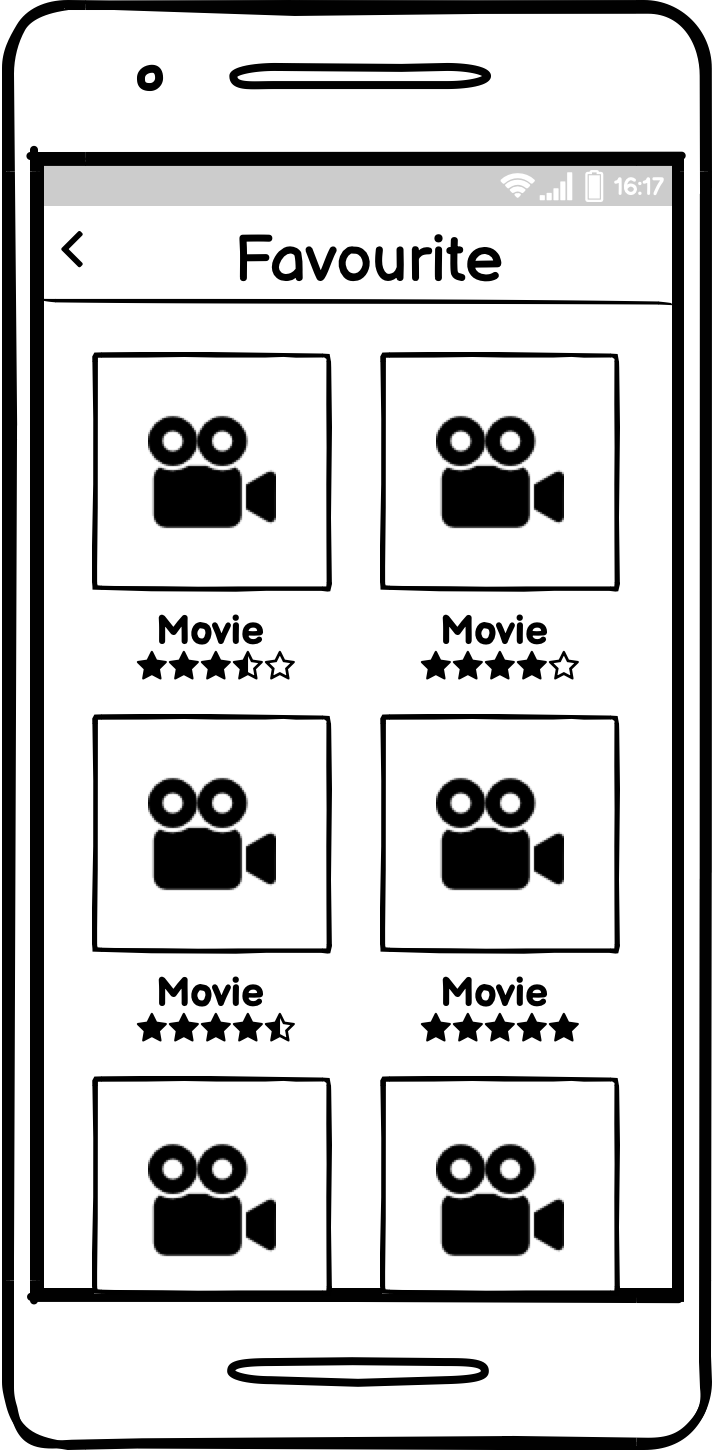
\includegraphics[width=0.68\textwidth]{images/mockups/Favourite.png}\\
			\caption{Favourite movie}
		\end{figure}
	\end{minipage}	
\end{center}
\mbox{}\\
\paragraph{Review a movie}
\mbox{}\\\\
The user can reach the review form in two ways:
\begin{itemize}
	\item from the movie page;
	\item from the reviews page.
\end{itemize}
As we can see in the following figure:
\begin{figure}[H]
	\centering
	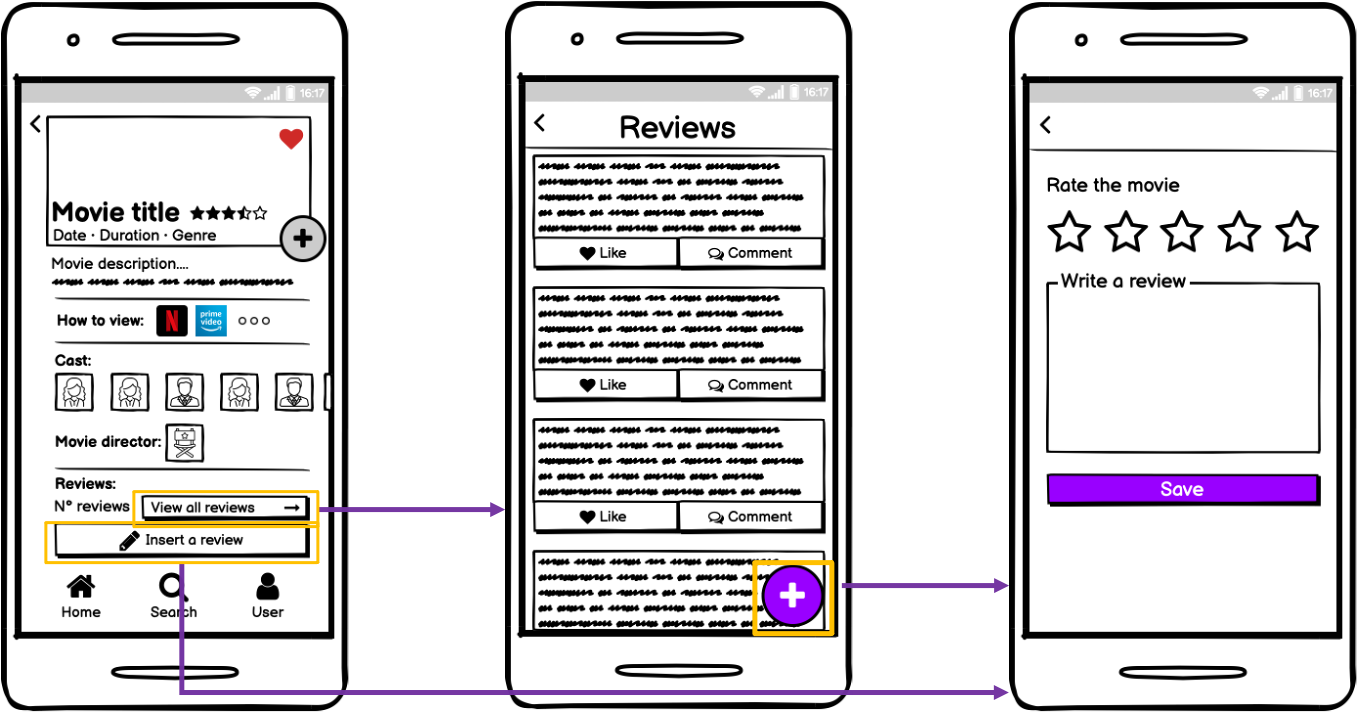
\includegraphics[width=0.9\textwidth]{images/mockups/review.png}\\
	\caption{How to make a review}
\end{figure}
\mbox{}\\\\
\paragraph{Comment other reviews}
\mbox{}\\\\
Tapping on "Comment" button, the user can see the comments of the other users and write a comment.
He can also tap on "Like" button in order to leave positive feedback regarding a certain review.
\begin{figure}[H]
	\centering
	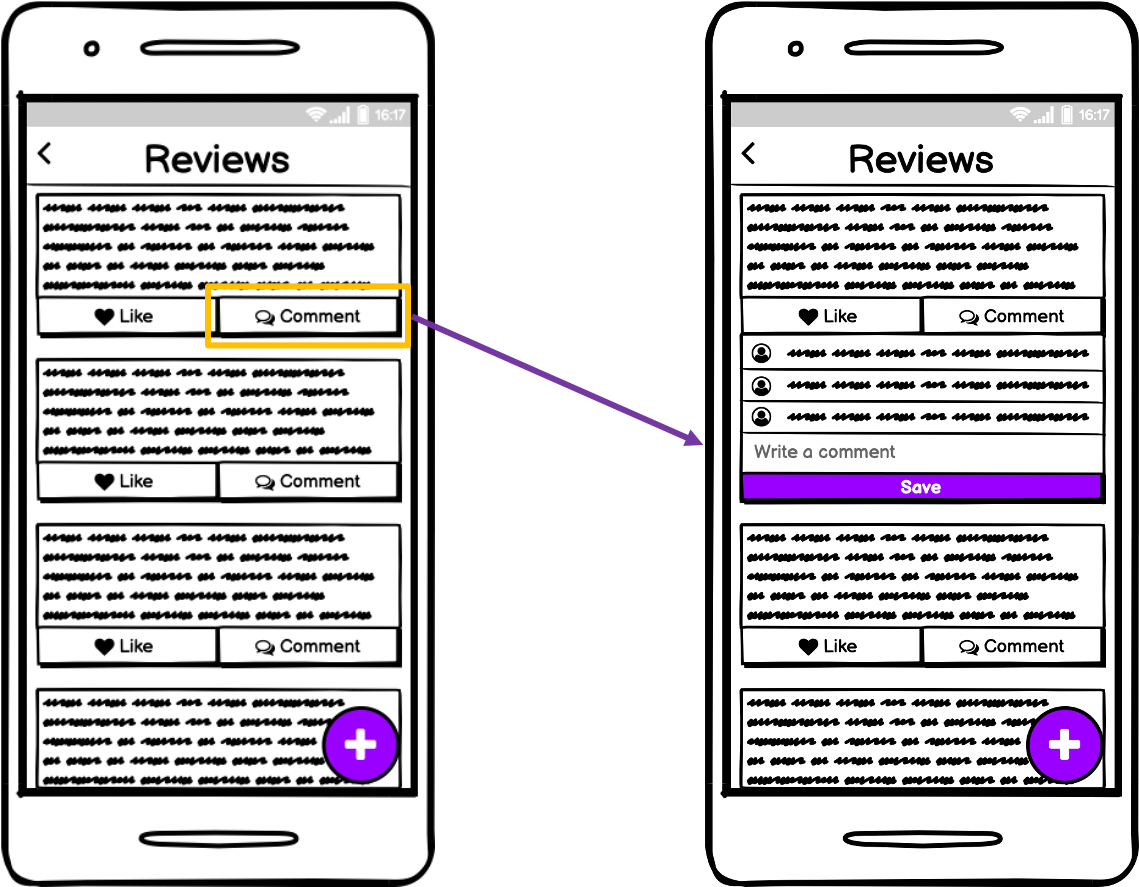
\includegraphics[width=0.6\textwidth]{images/mockups/comment.png}\\
	\caption{Comment other reviews process}
\end{figure}
\paragraph{User profile settings}
\mbox{}\\\\
Moreover, from the settings page, the user can change some profile settings like image profile, username and
password. Also, if the user has not done it before, he can link his profile with his Google or Facebook account.
Finally, here, the user can logout from the app.\\
These are not main functionalities, but we thought that they can be useful in order to support the user.
\begin{figure}[H]
	\centering
	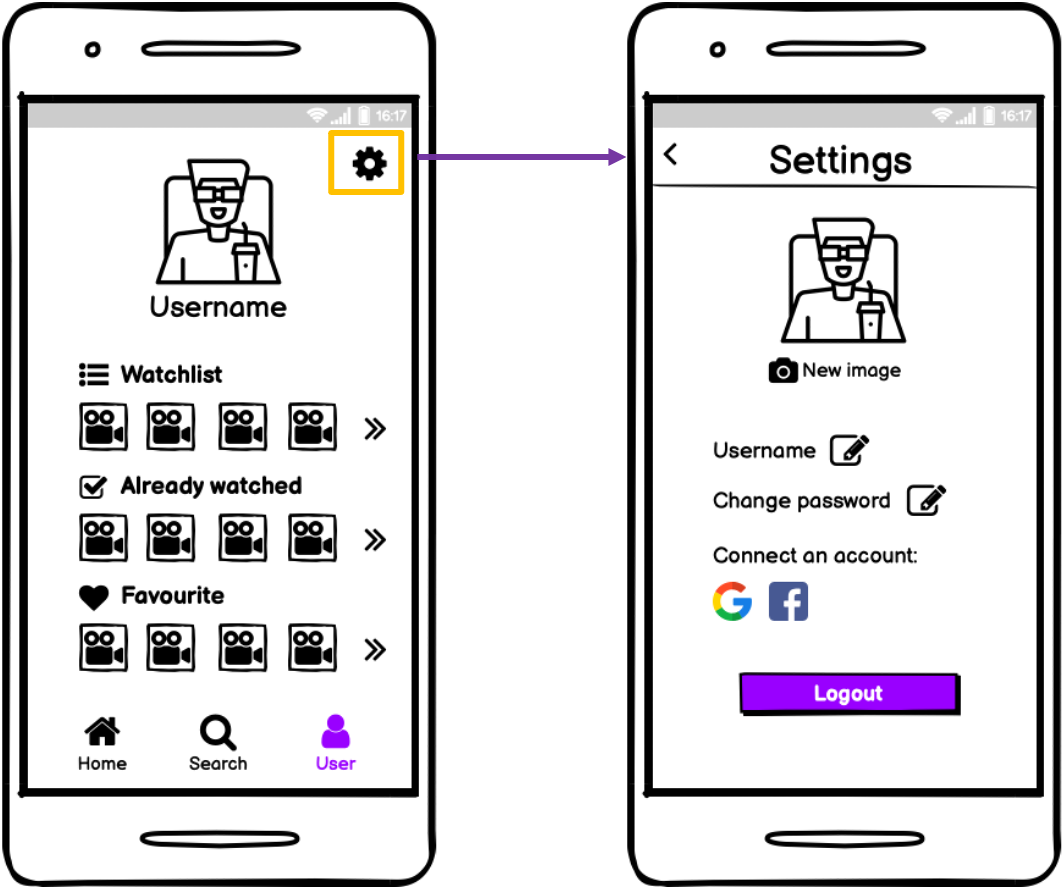
\includegraphics[width=0.6\textwidth]{images/mockups/userSettings.png}\\
	\caption{User profile and user profile settings pages}
\end{figure}
\begin{center}
	\begin{minipage}{0.3\textwidth}
		\begin{figure}[H]
			\centering
			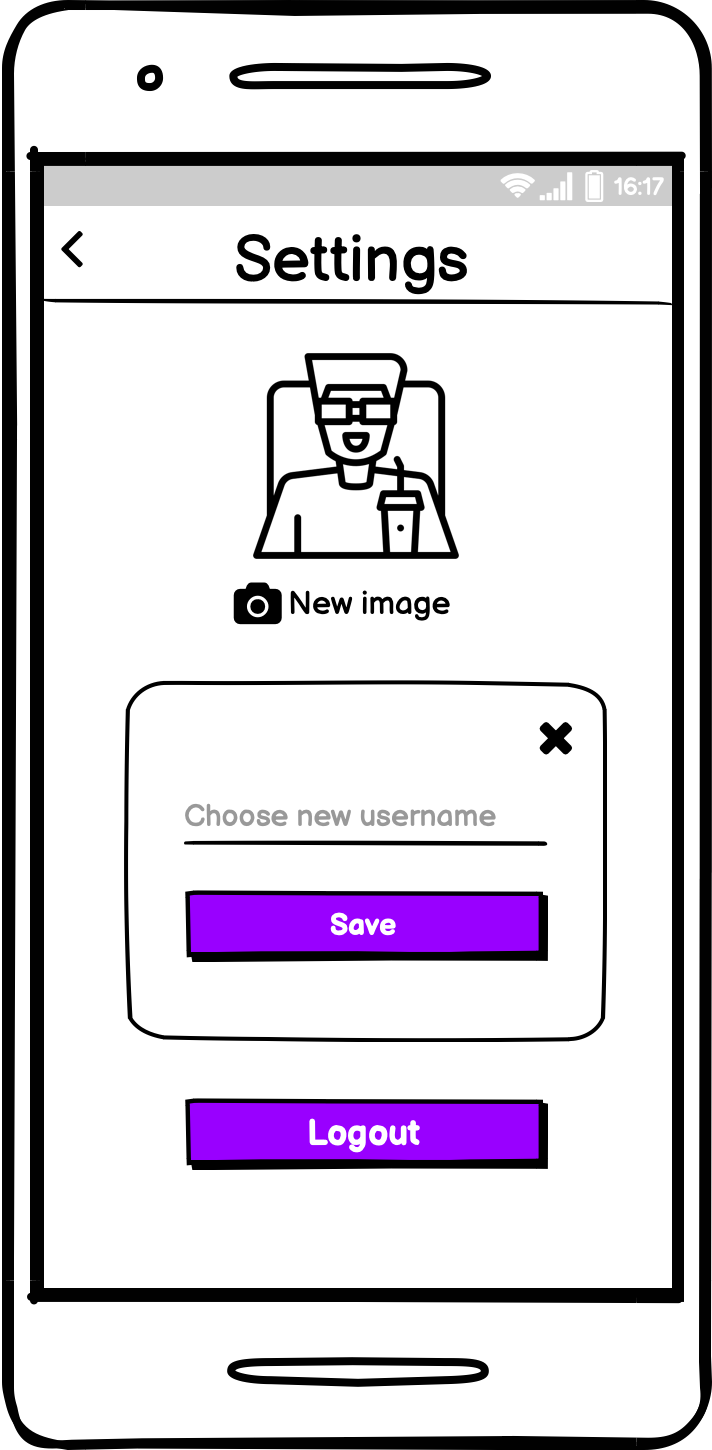
\includegraphics[width=0.8\textwidth]{images/mockups/User setting username.png}\\
			\caption{Change username}
		\end{figure}
	\end{minipage}
	\hspace{0.1\linewidth}
	\begin{minipage}{0.3\textwidth}
		\begin{figure}[H]
			\centering
			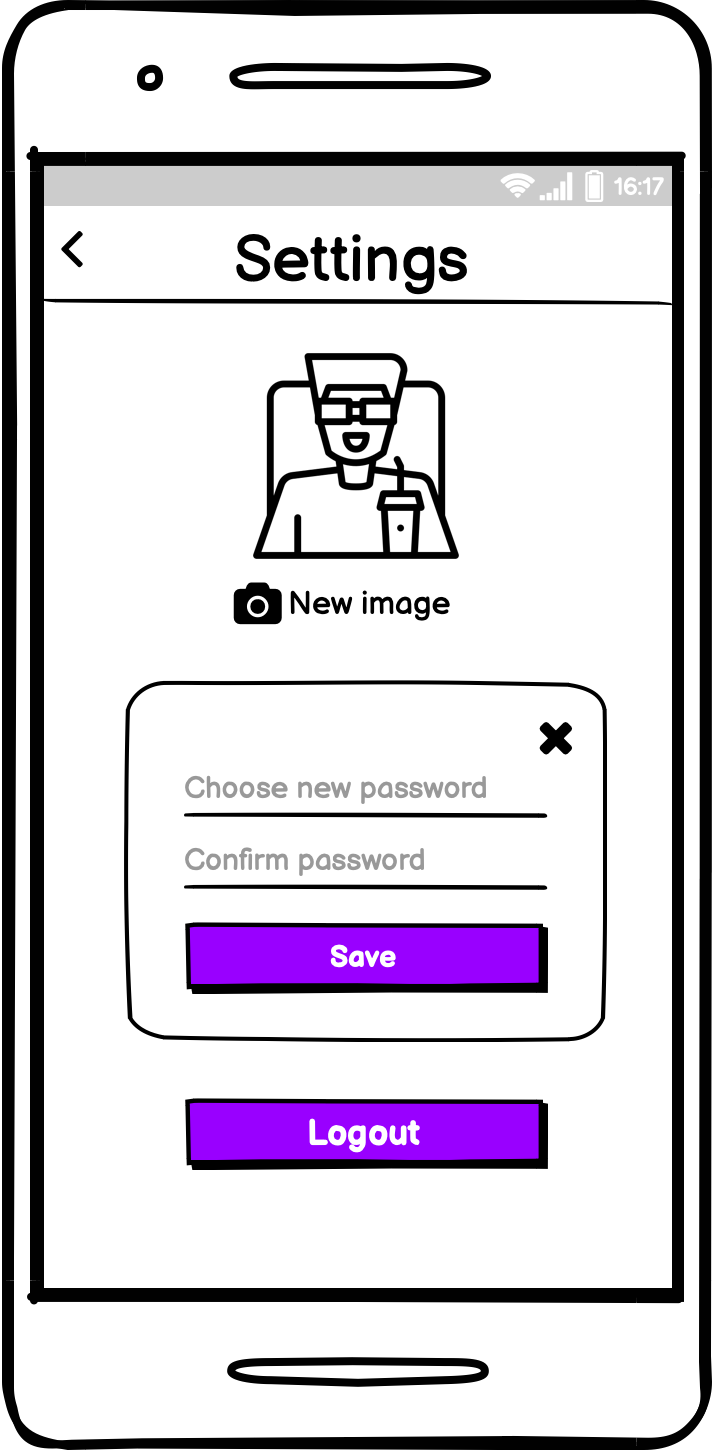
\includegraphics[width=0.8\textwidth]{images/mockups/User setting password.png}\\
			\caption{Change password}
		\end{figure}
	\end{minipage}	
\end{center}
\begin{center}
	\begin{minipage}{0.3\textwidth}
		\begin{figure}[H]
			\centering
			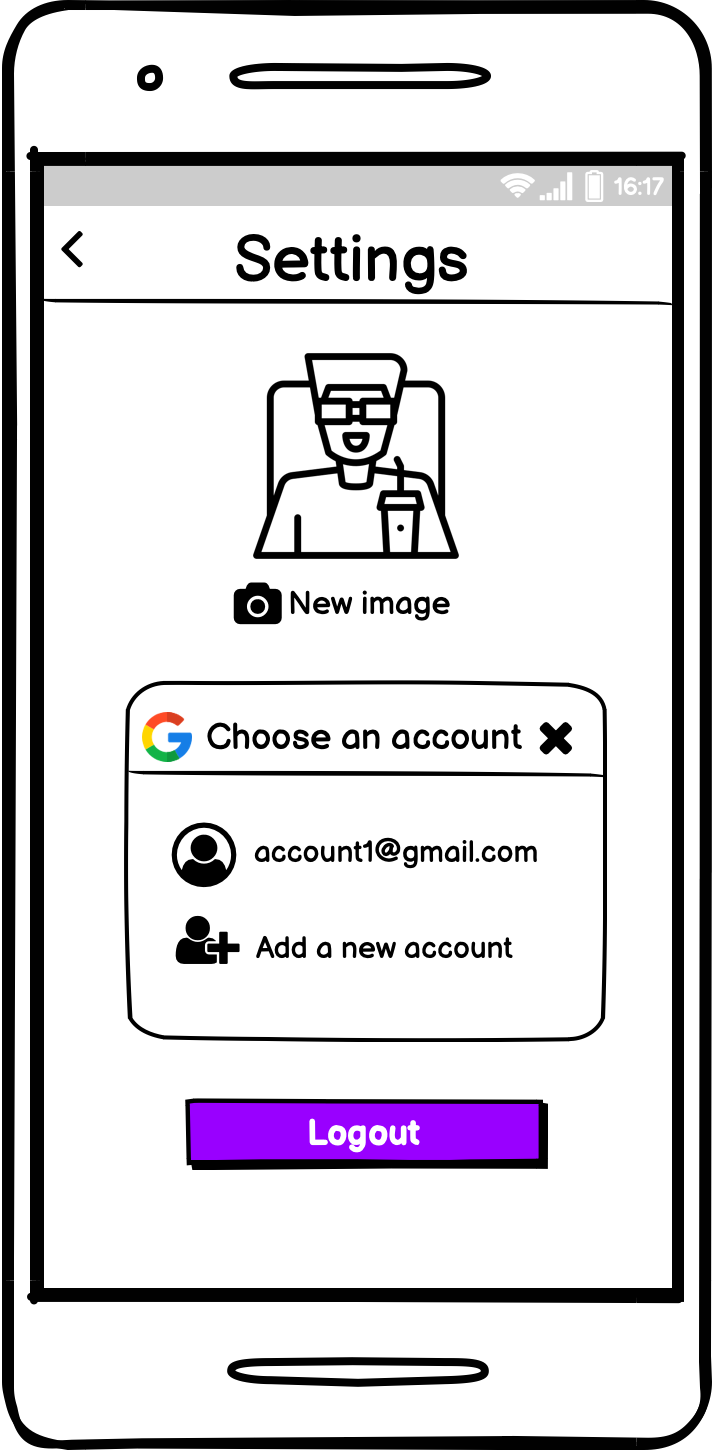
\includegraphics[width=0.8\textwidth]{images/mockups/User setting google.png}\\
			\caption{Connect google account}
		\end{figure}
	\end{minipage}
	\hspace{0.1\linewidth}
	\begin{minipage}{0.3\textwidth}
		\begin{figure}[H]
			\centering
			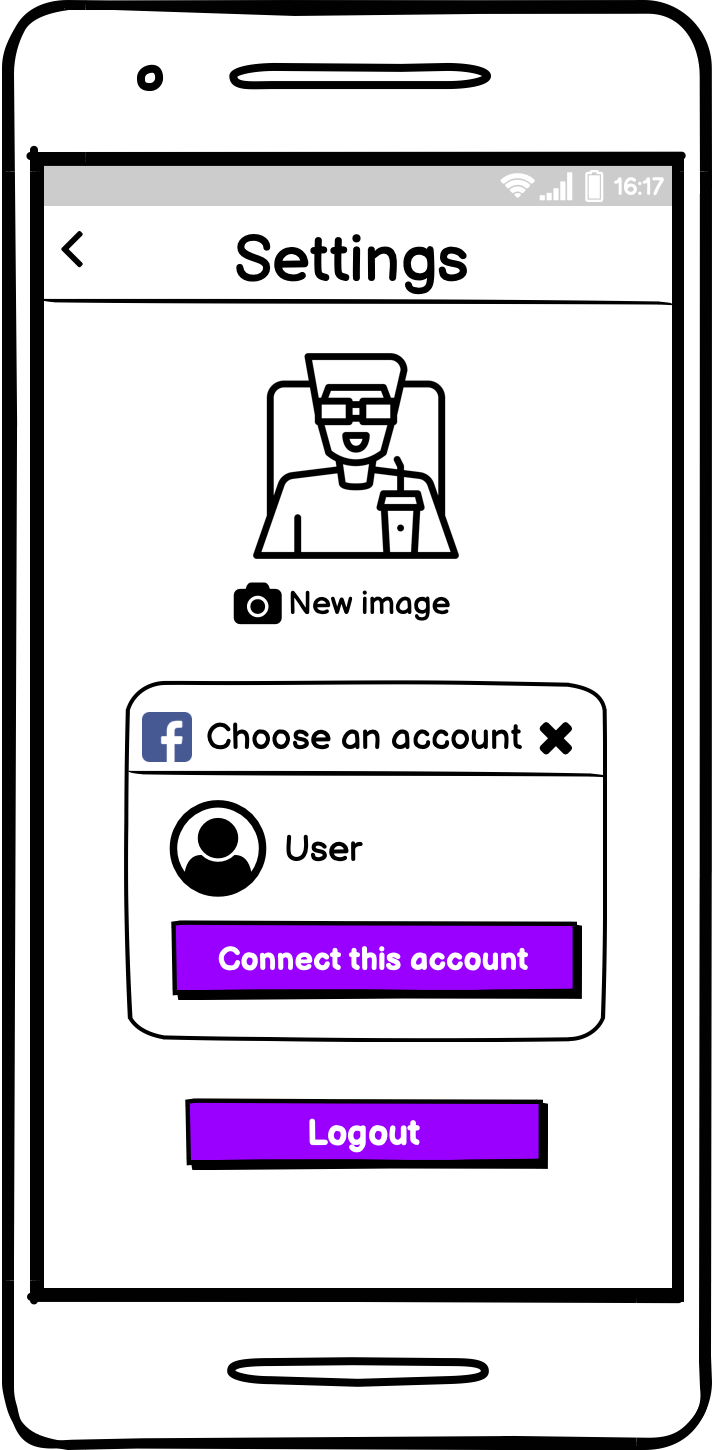
\includegraphics[width=0.8\textwidth]{images/mockups/User setting facebook.png}\\
			\caption{Connect facebook account}
		\end{figure}
	\end{minipage}	
\end{center}

% Expert Based Evaluation -------------------------------------------------------------------------

\newpage

\section{Expert Based Evaluation}
%TODO vedere se scritto bene che martina è incapace, non è all'altezza di valentown
The expert evaluation is based on our first prototype, the \textit{mockups} and it's really useful
for discovering problems. This is a very important thing to do until the implementation because
allow us to detects problems in early stage.\\\\
We submitted our \textit{mockups} on two different expert evaluation, made by professor Valeria Mirabella: 
\textbf{\textit{Heuristic Evaluation}} and \textbf{\textit{Cognitive Walkthrough}}.

\subsection{Heuristic Evaluation}
%TODO ho copiato da fly.ai -> modificare
Heuristic Evaluation is an inspection method used to evaluate if the system follows general usability 
criteria. The expert should check if the system is consistent and evaluates if the usability problem 
that may occurs is a major problem, a minor problem or just something that could be left as it is. 
The evaluation is made by assign severity level.
The main goal of heuristic evaluations is to identify any problem associated with the design of user interfaces.\\
The Heuristic Evaluation used is based on the Jakob Nielsen’s 10 Usability Heuristics:
\begin{enumerate}
	\item {\textit{Visibility of system status}: the system should always keep users informed about 
	what is going on, through appropriate feedback within reasonable time.}
	\item {\textit{Match between system and the real world}: the system should speak the users’ language,
	with words, phrases and concepts familiar to the user, rather than system-oriented terms. Follow 
	real-world conventions, making information appear in a natural and logical order.}
	\item {\textit{User control and freedom}: users often choose system functions by mistake and will 
	need a clearly marked ”emergency exit” to leave the unwanted state without having to go through an 
	extended dialogue. Support undo and redo.}
	\item {\textit{Consistency and standards}: users should not have to wonder whether different words, 
	situations, or actions mean the same thing. Follow platform conventions.}
	\item {\textit{Error prevention}: even better than good error messages is a careful design 
	which prevents a problem from occurring in the first place.}
	\item {\textit{Recognition rather than recall}: make objects, actions, and options visible. 
	The user should not have to remember information from one part of the dialogue to another. 
	Instructions for use of the system should be visible or easily retrievable.}
	\item {\textit{Flexibility and efficiency of use}: accelerators (unseen by the novice user) 
	may often speed up the interaction for the expert user such that the system can cater to both 
	inexperienced and experienced users. Allow users to tailor frequent actions.}
	\item {\textit{Aesthetic and minimalist design}: dialogues should not contain information which 
	is irrelevant or rarely needed. Every extra unit of information in a dialogue competes with the 
	relevant units of information and diminishes their relative visibility.}
	\item {\textit{Help users recognize, diagnose, and recover from errors}: error messages should 
	be expressed in plain language, precisely indicate the problem, and constructively suggest a 
	solution.}
	\item {\textit{Help and documentation}: even though it is better if the system can be used without 
	documentation, it may be necessary to provide help and documentation. Any such information should 
	be easy to search, focused on the user’s task, list concrete steps to be carried out, and not be 
	too large. whenever appropriate.}	 
\end{enumerate}
\mbox{}\\
\noindent
After the expert based evaluation, in the following table, it has been reported that the following 
heuristics have been violated:
\begin{figure}[H]
	\centering
	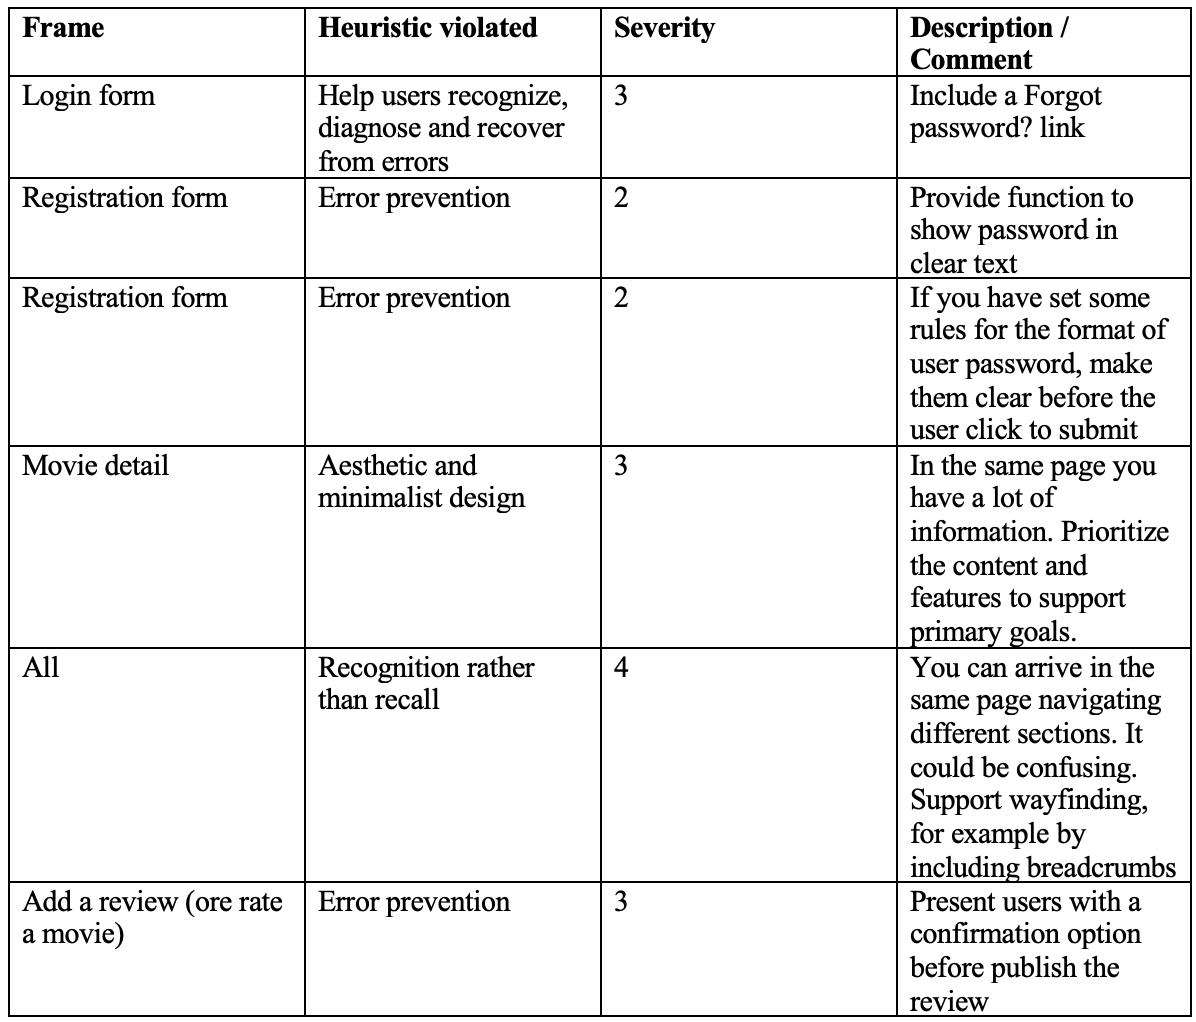
\includegraphics[width=1\textwidth]{images/heuristicEvaluation.png}\\
\end{figure}
\noindent
The severity number identify:
\begin{itemize}
	\item 0 = I don’t agree that this is a usability problem at all
	\item 1 = Cosmetic problem only
	\item 2 = Minor usability problem
	\item 3 = Major usability problem
	\item 4 = Usability catastrophe
\end{itemize}
\mbox{}\\\\\\\\\\
\subsection{Cognitive Walkthrough}
%TODO rivedere la definizione, l'ho copiata da fly.ai -> modificare
Cognitive Walkthrough is related with the idea of discover cognitive efforts of the user and how well 
the system supports the user executing the actions.
The idea of method provides the expert walks through the system in order to understand if the actions 
provided by the system well support the user in doing such task. 
The analysis is guided by four predefined questions:
\begin{itemize}
	\item Q1: Is the effect of the action the same as the user’s goal at that point?
	\item Q2: Will users see that the action is available?
	\item Q3: Once users have found the correct action, will they know it is the one they need?
	\item Q4: After the action is taken, will users understand the feedback they get?
\end{itemize}


\paragraph{Task 1 - Search the movie “Harry Potter and the Deathly Hallows - Part 2” to see the movie details.}\mbox{}\\\\
\textit{Action 1}: open the application (assuming that the user is already logged in)\\ 
\textit{Response 1}: homepage is opened\\
\textit{Action 2}: tap on the search icon\\
\textit{Response 2}: the search page is displayed\\
\textit{Action 3}: tap on the search bar\\
\textit{Response 3}: the keyboard shows up\\
\textit{Action 4}: type “Harry Potter”\\
\textit{Response 4}: each digit is displayed as typed and the system shows the corresponding results\\
\textit{Action 5 – 6 – 7}: [OPTIONAL] tap on filters’ icon, select “most recent” filter and tap on apply\\
\textit{Response 7}: the system shows the results according to the chosen filter\\
\textit{Action 8}: select “Harry Potter and the Deathly Hallows - Part 2” from the list of the results\\
\textit{Response 8}: the systems shows the page of the selected movie containing all the related details
\begin{figure}[H]
	\centering
	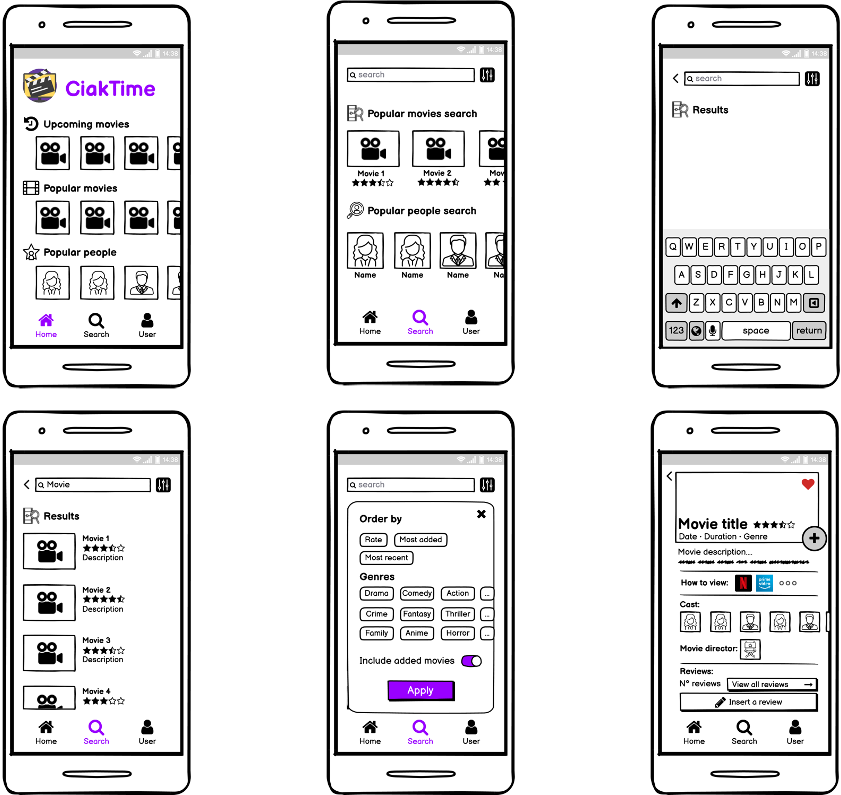
\includegraphics[width=0.7\textwidth]{images/mockupSearch.png}\\
\end{figure}
\noindent
Expert evaluation:\\\\
\textit{Action 1}: open the application (assuming that the user is already logged in)\\ 
\textit{Response 1}: homepage is opened\\\\
\textbf{Q1} - Is the effect of the action the same as the user’s goal at that point?\\
\tab Yes\\
\textbf{Q2} - Will users see that the action is available?\\
\tab Yes\\
\textbf{Q3} - Once users have found the correct action, will they know it is the one they need?\\
\tab Yes\\
\textbf{Q4} - After the action is taken, will users understand the feedback they get?\\
\tab Yes\\\\
\textit{Action 2}: tap on the search icon\\
\textit{Response 2}: the search page is displayed\\\\
\textbf{Q1} - Is the effect of the action the same as the user’s goal at that point?\\
\tab Yes\\
\textbf{Q2} - Will users see that the action is available?\\
\tab Yes\\
\textbf{Q3} - Once users have found the correct action, will they know it is the one they need?\\
\tab Yes\\
\textbf{Q4} - After the action is taken, will users understand the feedback they get?\\
\tab Yes\\\\
\textit{Action 3}: tap on the search bar\\
\textit{Response 3}: the keyboard shows up\\\\
\textbf{Q1} - Is the effect of the action the same as the user’s goal at that point?\\
\tab Yes\\
\textbf{Q2} - Will users see that the action is available?\\
\tab Yes\\
\textbf{Q3} - Once users have found the correct action, will they know it is the one they need?\\
\tab Yes\\
\textbf{Q4} - After the action is taken, will users understand the feedback they get?\\
\tab Yes\\\\
\textit{Action 4}: type “Harry Potter”\\
\textit{Response 4}: each digit is displayed as typed and the system shows the corresponding results\\\\
\textbf{Q1} - Is the effect of the action the same as the user’s goal at that point?\\
\tab Yes\\
\textbf{Q2} - Will users see that the action is available?\\
\tab Yes\\
\textbf{Q3} - Once users have found the correct action, will they know it is the one they need?\\
\tab Yes\\
\textbf{Q4} - After the action is taken, will users understand the feedback they get?\\
\tab Yes\\\\
\textit{Action 5 – 6 – 7}: [OPTIONAL] tap on filters’ icon, select “most recent” filter and tap on apply\\
\textit{Response 7}: the system shows the results according to the chosen filter\\\\
\textbf{Q1} - Is the effect of the action the same as the user’s goal at that point?\\
\tab Yes\\
\textbf{Q2} - Will users see that the action is available?\\
\tab Yes\\
\textbf{Q3} - Once users have found the correct action, will they know it is the one they need?\\
\tab Users with no experience could not recognize the icon\\
\textbf{Q4} - After the action is taken, will users understand the feedback they get?\\
\tab Yes\\\\
\textit{Action 8}: select “Harry Potter and the Deathly Hallows - Part 2” from the list of the results\\
\textit{Response 8}: the systems shows the page of the selected movie containing all the related details\\\\
\textbf{Q1} - Is the effect of the action the same as the user’s goal at that point?\\
\tab Yes\\
\textbf{Q2} - Will users see that the action is available?\\
\tab Yes\\
\textbf{Q3} - Once users have found the correct action, will they know it is the one they need?\\
\tab Yes\\
\textbf{Q4} - After the action is taken, will users understand the feedback they get?\\
\tab Yes\\\\


\paragraph{Task 2 - Add a popular movie to the watchlist.}\mbox{}\\\\
\textit{Action 1}: open the application (assuming that the user is already logged in)\\ 
\textit{Response 1}: homepage is opened\\
\textit{Action 2}: tap on a movie from “popular movies” section\\
\textit{Response 2}: the movies page is displayed\\
\textit{Action 3}: tap on the “+” button\\
\textit{Response 3}: lists’ popup is displayed\\
\textit{Action 4}: tap on watchlist\\
\textit{Response 4}: the movie is added to watchlist\\\\
\begin{figure}[H]
	\centering
	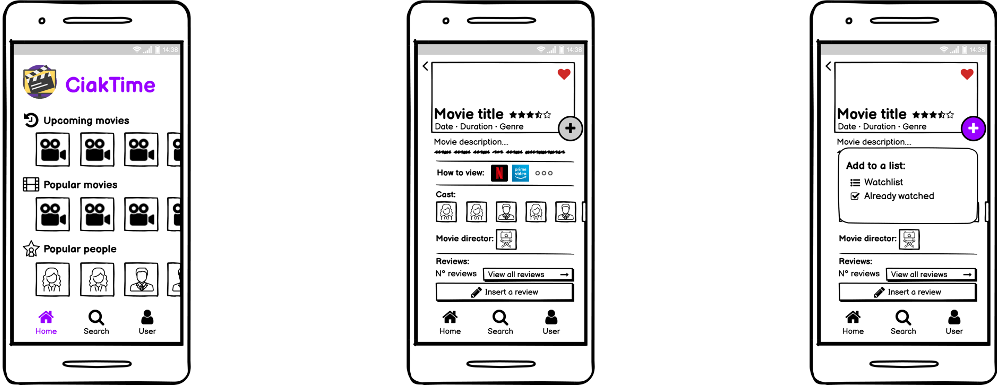
\includegraphics[width=0.9\textwidth]{images/mockupAdd.png}\\
\end{figure}
\mbox{}\\
\noindent
Expert evaluation:\\\\
\textit{Action 1}: open the application (assuming that the user is already logged in)\\ 
\textit{Response 1}: homepage is opened\\\\
\textbf{Q1} - Is the effect of the action the same as the user’s goal at that point?\\
\tab Yes\\
\textbf{Q2} - Will users see that the action is available?\\
\tab Yes\\
\textbf{Q3} - Once users have found the correct action, will they know it is the one they need?\\
\tab Yes\\
\textbf{Q4} - After the action is taken, will users understand the feedback they get?\\
\tab Yes\\\\
\textit{Action 2}: tap on a movie from “popular movies” section\\
\textit{Response 2}: the movies page is displayed\\\\
\textbf{Q1} - Is the effect of the action the same as the user’s goal at that point?\\
\tab Yes\\
\textbf{Q2} - Will users see that the action is available?\\
\tab Yes\\
\textbf{Q3} - Once users have found the correct action, will they know it is the one they need?\\
\tab Yes\\
\textbf{Q4} - After the action is taken, will users understand the feedback they get?\\
\tab Yes\\\\
\textit{Action 3}: tap on the “+” button\\
\textit{Response 3}: lists’ popup is displayed\\\\
\textbf{Q1} - Is the effect of the action the same as the user’s goal at that point?\\
\tab It could be not clear that the + button is needed to reach the goal\\
\textbf{Q2} - Will users see that the action is available?\\
\tab Yes\\
\textbf{Q3} - Once users have found the correct action, will they know it is the one they need?\\
\tab Yes\\
\textbf{Q4} - After the action is taken, will users understand the feedback they get?\\
\tab Yes\\\\
\textit{Action 4}: tap on watchlist\\
\textit{Response 4}: the movie is added to watchlist\\\\
\textbf{Q1} - Is the effect of the action the same as the user’s goal at that point?\\
\tab Yes\\
\textbf{Q2} - Will users see that the action is available?\\
\tab Yes\\
\textbf{Q3} - Once users have found the correct action, will they know it is the one they need?\\
\tab Yes\\
\textbf{Q4} - After the action is taken, will users understand the feedback they get?\\
\tab There aren't enough elements to answer\\\\

% Prototype 1 -------------------------------------------------------------------------

\newpage

\section{Prototype 1}
%TODO ho scritto una bozza. Per valentina: lo so che non sono all'altezza :c
After the expert evaluation, we do some corrections. 
In particular, regarding the heuristic evaluation abbiamo fatto qualche modifica
boh non so che scrivere\\
\paragraph{Login}
\mbox{}
\begin{figure}[H]
	\centering
	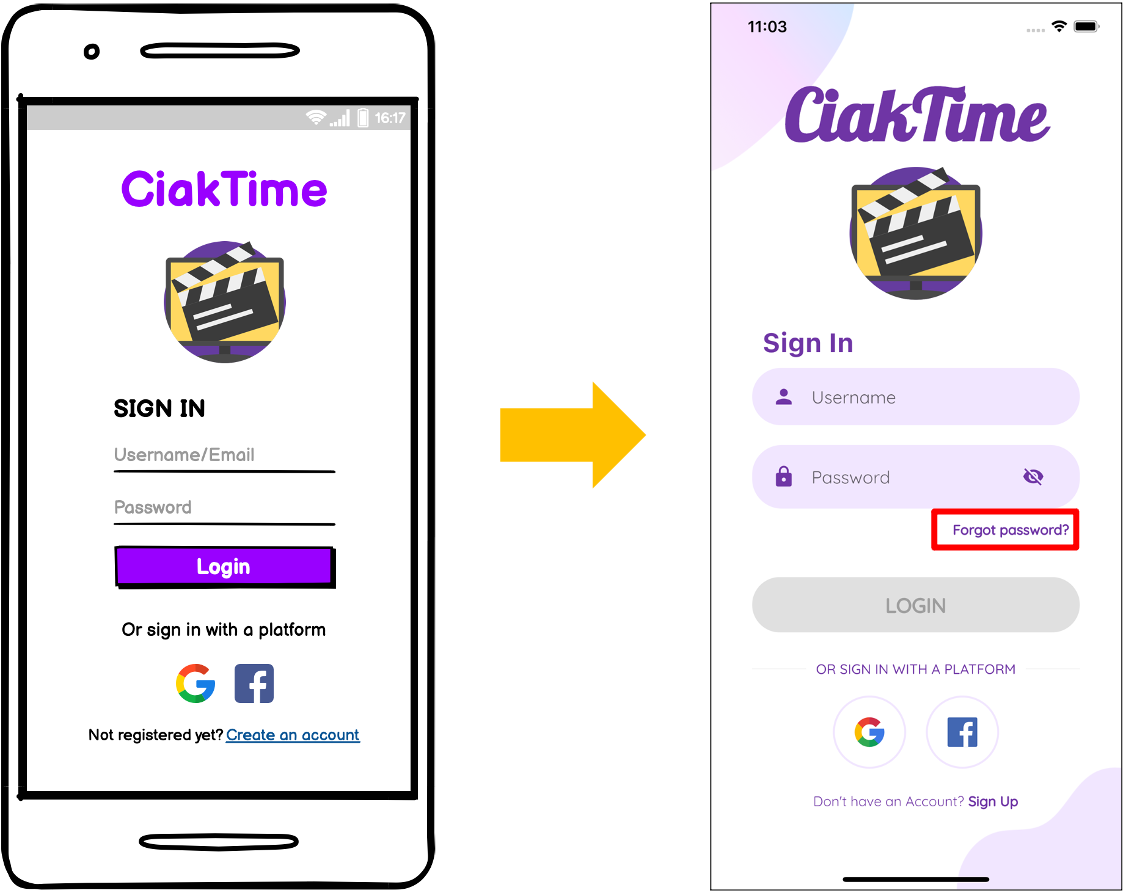
\includegraphics[width=0.7\textwidth]{images/prototype1/login.png}\\
	\caption{"Forgot password?" added to Login page}
\end{figure}
\paragraph{Registration}
\mbox{}
\begin{figure}[H]
	\centering
	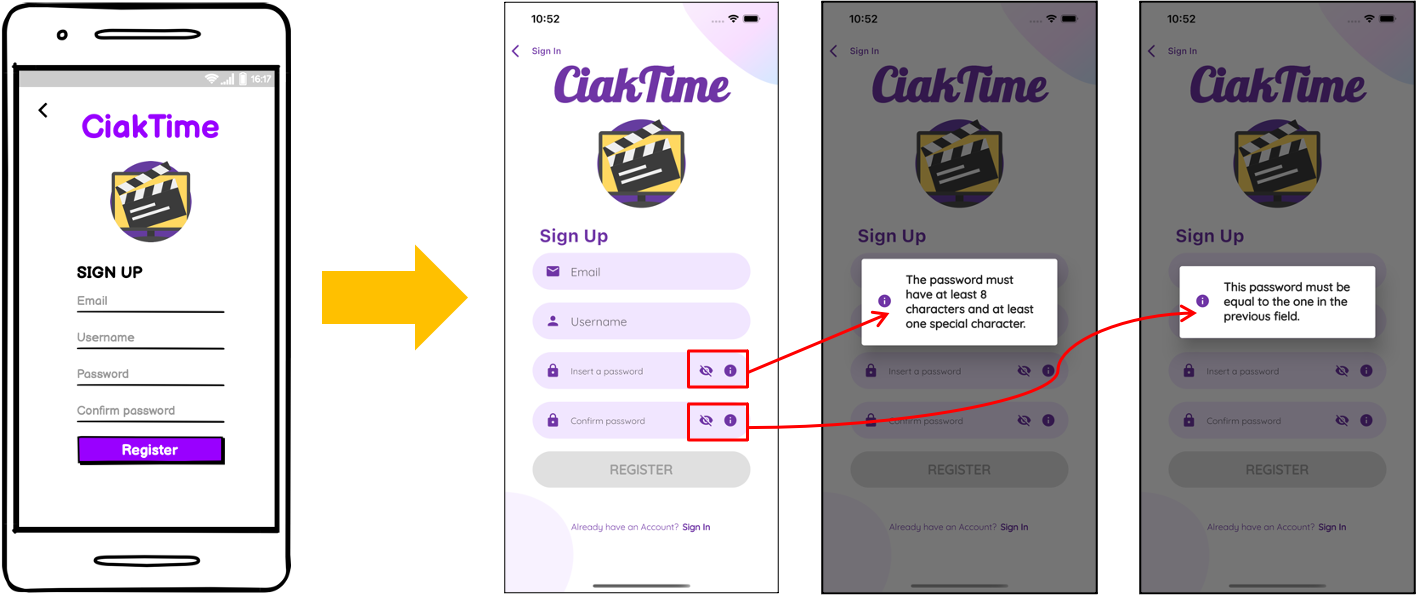
\includegraphics[width=1\textwidth]{images/prototype1/registration.png}\\
	\caption{Scrivere}
\end{figure}
\paragraph{Movie information}
\mbox{}
\begin{figure}[H]
	\centering
	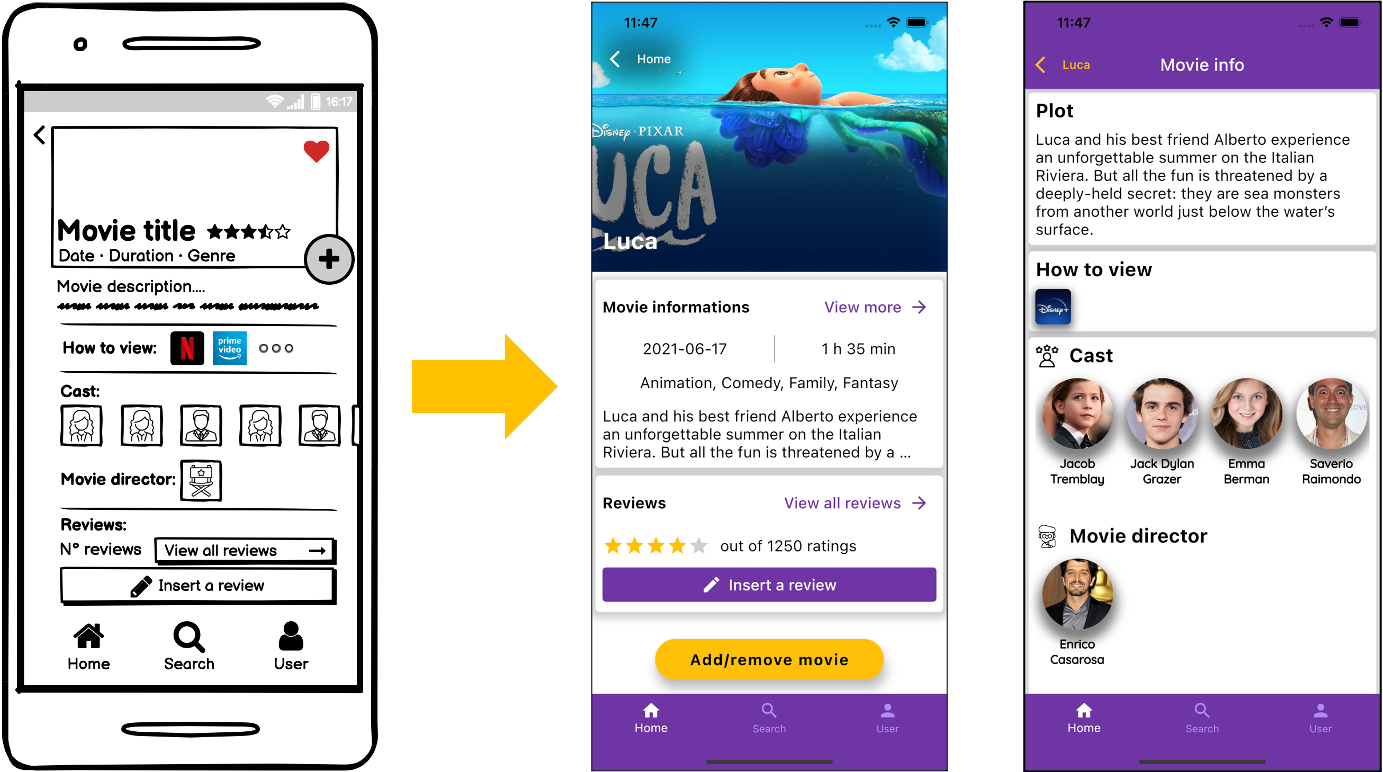
\includegraphics[width=1\textwidth]{images/prototype1/movieInfo.png}\\
	\caption{Scrivere}
\end{figure}

\noindent
Mettere correzioni basate sul Cognitive Walkthrough
\paragraph{Add movie to a list}
\mbox{}
\begin{figure}[H]
	\centering
	\includegraphics[width=0.7\textwidth]{images/prototype1/addBtn.png}\\
	\caption{Bottone di add btn modificato - scrivere}
\end{figure}
\begin{figure}[H]
	\centering
	\includegraphics[width=1\textwidth]{images/prototype1/addToList.png}\\
	\caption{Bottone di add btn modificato - scrivere}
\end{figure}

% User Based Evaluation -------------------------------------------------------------------------

\newpage

\section{User Based Evaluation}

Once Prototype 1 was up and running based on the corrections related to the expert evaluation, we 
proceeded with the user based evaluation. More precisely we used two techniques: \textbf{Think Aloud} and 
\textbf{Controlled experiment}.\\ These experiments were conducted over a group of subjects, representative 
of the future users, that did not participate in any of the previous phases.
Due to this emergency time that we are living, we exploited the functionality of Zoom that allowed us 
to connect with more people in order to have as much results as possible.\\
Our subjects had an age in a range between twenty - thirty years old that fits the age chosen in our user requirements.

\subsection{Think Aloud}

The think aloud is a kind of evaluation based on some simple rules. We chose a group of 10 people and 
performed the experiment using these criteria:
\begin{itemize}
	\item We explained to the users who we are and what we were doing.
	\item Each member had to accomplish, individually, the same tasks that are shown below.
	\item We explained that we were testing our application, and not testing them.
	\item The experiment took place remotely, and we provided a demo version of our app "CiakTime" to each person in order to allow them to install it on their smartphones.
	\item While executing the task, each user had to say aloud what he was doing, what he thought it was happening, any doubt, etc., and we were not allowed to help them in any way.
	\item During the experiment, we recorded each person and we took note by pen and paper.
\end{itemize}

\paragraph{Task 1:} \textit{Recently a lot of people are talking about the new Disney's movie called "Luca". So,  
in order to understand the reason behind that, you would like to read its plot. After having noticed that the plot is 
interesting, you would like to add that movie into your "Watchlist" in order to watch it in future.}

\paragraph{Task 2:} \textit{After having watched the movie "Luca", you would like to leave a review about this movie and 
add it to your "Already Watched" list.}

\paragraph{Task 3:} \textit{You really liked the movie "The lord of the rings: the fellowship of the ring" and you would know
who is the movie director and which other movies he has directed. After having done this search, you would like to go back
to the search page in order to do other searches.}

\mbox{}\\\\
Regarding \textit{Task 1}, some users, while performing this task, had some difficulties, because they tried to tap on 
the three dots at the end of the plot instead the "View more" button, in order to read the entire plot.
Conversely, regarding the other tasks, we notice that our subjects did not encounter any problem to accomplish them.\\
In general, we have obtained satisfactory results and therefore we asked the users to freely explore the application in order 
to collect additional advices to further improve it.\\
In particular, they made us notice that the comments page had not so many recalls to comment pages they were used to. 
In fact, in our comments page there were no references to the review they were linked to.


\subsection{Controlled experiment}


\begin{minipage}{0.3\textwidth}
	\begin{figure}[H]
		\centering
		\includegraphics[width=0.8\textwidth]{images/experiment/searchTab.png}\\
		\caption{Version 1}
	\end{figure}
\end{minipage}
\hspace{0.1\linewidth}
\begin{minipage}{0.3\textwidth}
	\textbf{Time:}\\\\
	100\\
	88\\
	65\\
	60\\
	90\\
	81\\
	110\\
	93\\
	87\\
	78\\
	\mbox{}\\\\\\\\\\\\
\end{minipage}
\mbox{}\\\\\\\\
\begin{minipage}{0.3\textwidth}
	\begin{figure}[H]
		\centering
		\includegraphics[width=0.8\textwidth]{images/experiment/searchCheckBox.png}\\
		\caption{Version 2}
	\end{figure}
\end{minipage}
\hspace{0.1\linewidth}
\begin{minipage}{0.3\textwidth}
	\textbf{Time:}\\\\
	100\\
	88\\
	65\\
	60\\
	90\\
	81\\
	110\\
	93\\
	87\\
	78\\
	\mbox{}\\\\\\\\\\\\
\end{minipage}


\paragraph{Task 1:} \textit{}

\subsubsection{ANOVA}

% CAPITOLO 7 -------------------------------------------------------------------------

\newpage

\section{Prototype 2: final prototype}

% CAPITOLO 8 -------------------------------------------------------------------------

\newpage

\section{NOME}

\end{document}

% COSE UTILI --------------------------------------------------------------------------

%\section*{NOME}
%\subsection*{1.1}
%\setlength{\intextsep}{0pt} --> elimina lo spazio
%\vspace{-3mm}
%\hspace*{0cm}

% Font -------------------------------------

%GRASSETTO: \textbf

% Simboli ---------------------------------

%$\leftarrow$

% Elenco puntato ----------------------

%\begin{itemize}
%\setlength\itemsep{0.01em}
%\item 1
%\item 2
%\end{itemize}

% Graffa grande -----------------------

%\[  
%    \left\{ 
%    \begin{array}{ll} 
%      \mbox{1}
%      \mbox{2}
%    \end{array}
%    \mbox{riga al lato}
%   \right. 
%\]

% Multicolonne --------------------------

% \begin{multicols}{2}
% \columnbreak
% \end{multicols}

% Algoritmi -------------------------------

%\renewcommand{\thealgorithm}{1.\arabic{algorithm}}
%\setcounter{algorithm}{0}
%\begin{algorithm}
%\footnotesize
%\caption{Nome}
%\textbf{Input:} \\
%\textbf{Output:} 

%\begin{algorithmic}[1]
%\STATE 
%\FOR{ = 0 \TO i = n} ---- \ENDFOR
%\IF{} ---- \ELSIF{} ---- \ENDIF
%\RETURN 
%\end{algorithmic}
%\end{algorithm}

% Minipage ------------------------------

%\begin{minipage}[t]{0.5\textwidth}

% queste 3 righe vanno attaccate
%\end{minipage}
%\hspace{0.02\linewidth}
%\begin{minipage}[t]{0.47\textwidth} 

%\begin{minipage}[t]{0.3\textwidth} 
%\end{minipage}

% Proof --------------------------------
%\begin{proof}[\textbf{per cambiare nome}]
%\end{proof}

